% Báo cáo cuối kỳ VN-Edu LOD (ontology 2.4) — biên dịch: latexmk -lualatex main.tex
% Số liệu/hình sinh tự động: python audit/release_metrics.py ; python docs/report/gen_tables.py ;
%                            python docs/report/gen_figures.py [--shots]
\documentclass[12pt,a4paper]{article}

% ---------------------------------------------------------------- ngôn ngữ, phông chữ, trang
\usepackage[vietnamese]{babel}
\usepackage{fontspec}
\setmainfont{Libertinus Serif}
\setsansfont{Libertinus Sans}
\setmonofont{Noto Sans Mono}[Scale=0.8]
\usepackage[section]{placeins}
\usepackage[a4paper,top=2.5cm,bottom=2.5cm,left=3cm,right=2cm]{geometry}
\usepackage{microtype}
\usepackage{setspace}
\setstretch{1.15}
\usepackage{amsmath,amssymb}
\usepackage{graphicx}
\usepackage{booktabs,tabularx,longtable,multirow,array}
\usepackage{xcolor}
\usepackage{enumitem}
\usepackage[font=small,labelfont=bf,labelsep=period]{caption}
\usepackage{subcaption}
\usepackage{rotating}
\usepackage{pdflscape}
\usepackage{fvextra}
\usepackage{tikz}
\usetikzlibrary{positioning,arrows.meta,shapes.geometric,fit,backgrounds,calc}
\usepackage{pgfplots}
\pgfplotsset{compat=1.18}
\usepackage[numbers,sort&compress]{natbib}
\usepackage[hidelinks]{hyperref}
\usepackage{xurl}
\usepackage[nameinlink]{cleveref}
\usepackage{fancyhdr}

\crefname{figure}{Hình}{Hình}
\crefname{table}{Bảng}{Bảng}
\crefname{section}{Mục}{Mục}
\crefname{subsection}{Mục}{Mục}
\crefname{subsubsection}{Mục}{Mục}
\crefname{appendix}{Phụ lục}{Phụ lục}
\crefname{listing}{Đoạn mã}{Đoạn mã}
\newcommand{\crefpairconjunction}{ và }
\newcommand{\crefmiddleconjunction}{, }
\newcommand{\creflastconjunction}{ và }
\newcommand{\crefrangeconjunction}{--}
\addto\captionsvietnamese{%
  \renewcommand{\figurename}{Hình}\renewcommand{\tablename}{Bảng}%
  \renewcommand{\contentsname}{Mục lục}\renewcommand{\listfigurename}{Danh mục hình}%
  \renewcommand{\listtablename}{Danh mục bảng}\renewcommand{\refname}{Tài liệu tham khảo}%
  \renewcommand{\abstractname}{Tóm tắt}\renewcommand{\appendixname}{Phụ lục}}

\definecolor{acc}{HTML}{0F6E64}
\definecolor{s1}{HTML}{2A78D6}
\definecolor{s2}{HTML}{EB6834}
\definecolor{s3}{HTML}{1BAF7A}
\definecolor{s4}{HTML}{8C939C}
\definecolor{bronze}{HTML}{B07A4A}
\definecolor{silver}{HTML}{8C939C}
\definecolor{gold}{HTML}{C9A227}

\setlist{itemsep=2pt,topsep=4pt}
\setlength{\parskip}{4pt}
\setlength{\emergencystretch}{5em}
\tolerance=2000
\renewcommand{\arraystretch}{1.15}
\pagestyle{fancy}\fancyhf{}\fancyhead[L]{\small VN-Edu LOD}\fancyhead[R]{\small Báo cáo cuối kỳ -- Web ngữ nghĩa}\fancyfoot[C]{\thepage}
\setlength{\headheight}{15pt}

\DefineVerbatimEnvironment{code}{Verbatim}{fontsize=\footnotesize, frame=single, rulecolor=\color{black!20},
  framesep=2.5mm, breaklines=true, breakanywhere=true}
\newcommand{\codetitle}[1]{\par\smallskip\noindent{\small\bfseries #1}\par\nopagebreak}
\newcommand{\vn}[1]{\texttt{vnedu:\allowbreak #1}}
\newcommand{\proj}{VN-Edu LOD}
\newcommand{\RQ}[1]{\textbf{RQ#1}}
\newcommand{\CQ}[1]{\textbf{CQ#1}}

% Generated by audit/release_metrics.py
\newcommand{\metricInstitutions}{297}
\newcommand{\metricHEIs}{268}
\newcommand{\metricPeople}{1{,}703}
\newcommand{\metricLeaders}{221}
\newcommand{\metricAlumni}{0}
\newcommand{\metricEducationParticipants}{1{,}482}
\newcommand{\metricObservations}{4{,}165}
\newcommand{\metricPrograms}{78}
\newcommand{\metricMajors}{37}
\newcommand{\metricCurrentProvinces}{34}
\newcommand{\metricFormerProvinces}{29}
\newcommand{\metricAssertedTriples}{59{,}392}
\newcommand{\metricInferredTriples}{23{,}014}
\newcommand{\metricLinkTriples}{3{,}557}
\newcommand{\metricOsmCoordinateTriples}{126}
\newcommand{\metricOntologyTriples}{948}
\newcommand{\metricUnionTriples}{87{,}162}
\newcommand{\metricMetadataTriples}{129}
\newcommand{\metricLocalResources}{6{,}413}
\newcommand{\metricClasses}{44}
\newcommand{\metricObjectProperties}{40}
\newcommand{\metricDataProperties}{29}
\newcommand{\metricFoundingConflicts}{5}
\newcommand{\metricWarnings}{33}
\newcommand{\metricViolations}{0}
\newcommand{\metricInformationResults}{1}

% Sinh tự động bởi docs/report/gen_figures.py — không sửa tay
\newcommand{\stBacPub}{112}
\newcommand{\stBacPri}{10}
\newcommand{\stBacRel}{1}
\newcommand{\stBacUnk}{6}
\newcommand{\stTrungPub}{37}
\newcommand{\stTrungPri}{6}
\newcommand{\stTrungRel}{0}
\newcommand{\stTrungUnk}{3}
\newcommand{\stNamPub}{54}
\newcommand{\stNamPri}{16}
\newcommand{\stNamRel}{0}
\newcommand{\stNamUnk}{6}
\newcommand{\stDecades}{(1890,2) (1900,9) (1910,1) (1920,2) (1940,10) (1950,49) (1960,42) (1970,34) (1980,5) (1990,28) (2000,56) (2010,19) (2020,2)}
\newcommand{\stLinkWikidata}{1885}
\newcommand{\stLinkWikipedia}{1186}
\newcommand{\stLinkDBpedia}{228}
\newcommand{\stLinkROR}{195}
\newcommand{\stLinkGeoNames}{63}
\newcommand{\stActiveHEI}{258}


% ---------------------------------------------------------------- kiểu hình TikZ
\tikzset{
  box/.style={draw=#1!80!black, fill=#1!10, rounded corners=3pt, thick, align=center, font=\small,
              inner sep=4pt, text width=2.6cm, minimum height=1.0cm},
  box/.default=black,
  wide/.style={box=#1, text width=3.5cm},
  layer/.style={draw=black!25, fill=black!2, rounded corners=6pt, inner sep=7pt},
  ltitle/.style={font=\small\bfseries\scshape, text=black!65},
  flow/.style={-{Stealth[length=2.5mm]}, thick, draw=black!65},
  dflow/.style={-{Stealth[length=2.5mm]}, thick, densely dashed, draw=black!50},
  db/.style={cylinder, shape border rotate=90, aspect=0.2, draw=#1!80!black, fill=#1!10, thick, align=center,
             font=\small, minimum width=2.4cm, minimum height=1.2cm, inner sep=2pt},
}

\hypersetup{pdftitle={VN-Edu LOD: Bộ dữ liệu liên kết mở 5 sao về giáo dục đại học Việt Nam}, pdfauthor={[Họ và tên]}}

\begin{document}

% ================================================================= trang bìa
\begin{titlepage}
\thispagestyle{empty}
\centering
{\large\bfseries [TÊN TRƯỜNG ĐẠI HỌC]\par}
{\large [TÊN KHOA / VIỆN]\par}
\vspace{0.3cm}\rule{0.55\textwidth}{0.4pt}\par
\vspace{2.2cm}
{\Large\bfseries BÁO CÁO CUỐI KỲ\par}
\vspace{0.3cm}
{\large Học phần: Web ngữ nghĩa (Semantic Web) \quad Mã học phần: [Mã HP]\par}
\vspace{1.6cm}
{\LARGE\bfseries VN-Edu LOD\par}
\vspace{0.4cm}
{\Large\bfseries XÂY DỰNG ỨNG DỤNG DỮ LIỆU LIÊN KẾT MỞ 5 SAO\\[3pt] VỀ CÁC CƠ SỞ GIÁO DỤC ĐẠI HỌC VIỆT NAM\par}
\vspace{0.5cm}
{\large Thiết kế ontology OWL 2, tích hợp đa nguồn theo kiến trúc Medallion,\\ suy luận, kiểm định chất lượng
và công bố trên Web\par}
\vspace{2.0cm}
\begin{tabular}{rl}
Sinh viên thực hiện: & [Họ và tên] \\
Mã số sinh viên:    & [MSSV] \\
Lớp:                & [Lớp] \\[6pt]
Giảng viên hướng dẫn: & [Họ tên giảng viên] \\
\end{tabular}
\vfill
{\small
\begin{tabular}{rl}
Trang dữ liệu (tĩnh): & \url{https://pham-ng.github.io/Vietnam-University-Knowledge-Graph-ver2/} \\
SPARQL endpoint:      & \url{https://vnedu-lod.onrender.com/sparql} \\
Mã nguồn:             & \url{https://github.com/pham-ng/Vietnam-University-Knowledge-Graph-ver2} \\
\end{tabular}}
\vspace{0.9cm}

{\large [Thành phố], tháng 10 năm 2026\par}
\end{titlepage}

% ================================================================= tóm tắt
\pagenumbering{roman}
\begin{abstract}
\noindent Thông tin về hệ thống giáo dục đại học Việt Nam hiện phân tán ở nhiều nguồn: cổng tuyển sinh của Bộ Giáo
dục và Đào tạo, Wikipedia tiếng Việt, Wikidata, DBpedia, Research Organization Registry (ROR) và các văn bản quy phạm
pháp luật. Các nguồn này khác nhau về định dạng, mức độ đầy đủ và đều không có ngữ nghĩa máy đọc được. Báo cáo này
trình bày \proj{}, một ứng dụng dữ liệu liên kết mở (Linked Open Data -- LOD) đạt chuẩn 5 sao của Tim
Berners-Lee~\cite{bernerslee2006linked} về các cơ sở giáo dục đại học Việt Nam. Chúng tôi (i) thiết kế ontology
\texttt{vnedu:} phiên bản 2.4 gồm \metricClasses{} lớp, \metricObjectProperties{} thuộc tính đối tượng và
\metricDataProperties{} thuộc tính dữ liệu, nằm trong hồ sơ OWL~2~RL và OWL~2~DL; (ii) xây dựng một pipeline tái lập được
theo kiến trúc Medallion (Bronze--Silver--Gold) để tích hợp 8 nguồn dữ liệu; (iii) liên kết tới Wikidata, DBpedia, ROR,
GeoNames và Wikipedia bằng \metricLinkTriples{} triple liên kết; (iv) suy luận OWL~2~RL và kiểm định SHACL; (v) công bố
dữ liệu bằng URI có thể tra cứu (dereferenceable) với thương lượng nội dung, một SPARQL endpoint công khai và một trang
web tĩnh có bộ máy truy vấn chạy ngay trong trình duyệt. Đồ thị công bố có \metricUnionTriples{} triple, mô tả
\metricInstitutions{} cơ sở giáo dục (\metricHEIs{} cơ sở giáo dục đại học), \metricPeople{} cá nhân và 63 đơn vị hành
chính cấp tỉnh trước và sau sắp xếp năm 2025. Kết quả đánh giá cho thấy: 0 vi phạm SHACL, HermiT xác nhận ontology nhất
quán, độ chính xác liên kết \(100/100\) trên mẫu kiểm tra thủ công (khoảng tin cậy Wilson 95\%: 96,3--100\%), và hai
lần chạy pipeline ngoại tuyến liên tiếp sinh ra dữ liệu giống nhau đến từng byte.

\medskip\noindent\textbf{Từ khoá:} Linked Open Data, Semantic Web, ontology, OWL 2 RL, SHACL, SPARQL, knowledge graph,
giáo dục đại học Việt Nam.
\end{abstract}

\clearpage
\tableofcontents
\clearpage
\listoffigures
\listoftables
\clearpage
\pagenumbering{arabic}

% ================================================================= 1. GIỚI THIỆU
\section{Giới thiệu}\label{sec:intro}

\subsection{Bối cảnh và động lực}
Việt Nam có hơn 250 cơ sở giáo dục đại học đang hoạt động. Mỗi cơ sở thuộc một trong nhiều loại hình (đại học quốc
gia, đại học vùng, đại học, học viện, trường đại học, trường sĩ quan) và chịu sự quản lý của nhiều loại cơ quan chủ
quản (Bộ Giáo dục và Đào tạo, các bộ ngành khác, Uỷ ban nhân dân cấp tỉnh, tổ chức chính trị -- xã hội). Năm 2025,
Nghị quyết 202/2025/QH15~\cite{vn2025nq202} sắp xếp 63 tỉnh thành còn 34, khiến địa chỉ hành chính của phần lớn cơ sở ghi
trong các nguồn trước đó trở nên lỗi thời.

Người học, nhà nghiên cứu và nhà quản lý thường cần trả lời những câu hỏi như: ``Tỉnh nào sau sáp nhập có nhiều trường
đại học nhất?'', ``Những trường nào thuộc khối quân đội hoặc công an?'', ``Ai đang là hiệu trưởng trường X và người đó
từng học ở đâu?''. Hiện nay, trả lời các câu hỏi này đòi hỏi tra cứu thủ công trên nhiều trang web. Các nguồn mở như
Wikidata hay DBpedia~\cite{vrandecic2014wikidata,lehmann2015dbpedia} có mô hình hoá các trường đại học Việt Nam nhưng
không đầy đủ và không phản ánh các khái niệm đặc thù của Việt Nam, như cơ quan chủ quản, mã tuyển sinh hay tỉnh mới
sau sáp nhập.

Dữ liệu liên kết (Linked Data)~\cite{bizer2009linked,heath2011linked} cho phép giải quyết vấn đề này: mỗi thực thể có
một URI HTTP toàn cục, được mô tả bằng RDF theo một ontology chung và liên kết tới các bộ dữ liệu khác. Nhờ vậy, máy có
thể tích hợp dữ liệu, suy luận và truy vấn thống nhất qua SPARQL.

\subsection{Mục tiêu và câu hỏi nghiên cứu}
Đồ án đặt mục tiêu \emph{xây dựng một ứng dụng LOD đạt chuẩn 5 sao cho miền giáo dục đại học Việt Nam}. Ba câu hỏi
nghiên cứu sau định hướng thiết kế và đánh giá:

\begin{description}[leftmargin=1.2cm,style=nextline]
  \item[\RQ{1}] Có thể thiết kế một ontology vừa đủ biểu đạt các khái niệm đặc thù của Việt Nam (cơ quan chủ quản, loại
  hình sở hữu, địa giới hành chính trước và sau 2025, lãnh đạo, ngành đào tạo), vừa nằm trong hồ sơ OWL~2~RL để suy
  luận được ở quy mô toàn bộ dữ liệu không?
  \item[\RQ{2}] Có thể tích hợp dữ liệu từ nhiều nguồn có chất lượng không đồng đều một cách \emph{tái lập được} và
  \emph{truy vết được nguồn gốc} (provenance), sao cho mỗi khẳng định đều có nguồn và những mâu thuẫn được giữ lại thay
  vì bị che giấu không?
  \item[\RQ{3}] Bộ dữ liệu có đạt đủ 5 tiêu chí LOD, với liên kết ra ngoài có độ chính xác cao và các dịch vụ truy cập
  (URI tra cứu được, SPARQL) đủ dùng trên hạ tầng miễn phí không?
\end{description}

\subsection{Đóng góp}
\begin{enumerate}
  \item Ontology \texttt{vnedu:} 2.4 (\cref{sec:ontology}) gồm \metricClasses{} lớp chia thành 5 mô-đun, căn chỉnh với
  schema.org, DBpedia, FOAF, PROV-O và SKOS, đạt 0 vi phạm hồ sơ OWL~2~RL và OWL~2~DL, được HermiT xác nhận nhất quán.
  \item Pipeline Medallion 7 bước (\cref{sec:arch,sec:data}) có bộ đệm HTTP đóng gói, cho phép xây lại toàn bộ dữ liệu
  ngoại tuyến và ra kết quả giống nhau đến từng byte.
  \item Mô hình quan sát có nguồn gốc (\vn{SourceObservation}) để ghi lại nguồn, thời điểm và mâu thuẫn giữa các nguồn
  mà không khẳng định sai sự thật hiện tại.
  \item Đồ thị tri thức \metricUnionTriples{} triple với \metricLinkTriples{} liên kết ra ngoài, được đánh giá định
  lượng về độ chính xác (\cref{sec:eval}).
  \item Hạ tầng công bố hai kênh (\cref{sec:publish}): web tĩnh trên GitHub Pages kèm SPARQL chạy trong trình duyệt
  (Oxigraph/WASM), và máy chủ Linked Data trên Render với thương lượng nội dung và SPARQL endpoint chuẩn W3C.
\end{enumerate}

\subsection{Cấu trúc báo cáo}
\Cref{sec:background} trình bày cơ sở lý thuyết và các công trình liên quan. \Cref{sec:req} phân tích yêu cầu và nguồn
dữ liệu. \Cref{sec:arch} mô tả kiến trúc hệ thống. \Cref{sec:ontology} trình bày thiết kế ontology. \Cref{sec:data} mô
tả quy trình xây dựng dữ liệu và liên kết. \Cref{sec:reason} trình bày suy luận và kiểm định chất lượng. \Cref{sec:publish}
mô tả công bố và ứng dụng. \Cref{sec:eval} đánh giá kết quả. \Cref{sec:discussion} thảo luận hạn chế, và
\cref{sec:conclusion} kết luận.

% ================================================================= 2. CƠ SỞ LÝ THUYẾT
\section{Cơ sở lý thuyết và công trình liên quan}\label{sec:background}

\subsection{Dữ liệu liên kết và thang 5 sao}
Berners-Lee~\cite{bernerslee2006linked} đưa ra bốn nguyên tắc của Linked Data: (1) dùng URI để định danh sự vật;
(2) dùng URI HTTP để có thể tra cứu; (3) khi URI được tra cứu, trả về thông tin hữu ích theo chuẩn (RDF, SPARQL);
(4) liên kết tới URI khác để khám phá thêm. Thang 5 sao xếp hạng dữ liệu mở như ở \cref{tab:5star}.

\begin{table}[htbp]
\centering\small
\caption{Thang 5 sao của dữ liệu mở và cách \proj{} đáp ứng từng tiêu chí.}\label{tab:5star}
\begin{tabularx}{\textwidth}{c>{\raggedright\arraybackslash}p{4.2cm}X}
\toprule
Mức & Tiêu chí & Cách đáp ứng trong \proj{} \\
\midrule
\(\star\) & Công bố trên Web với giấy phép mở & Dữ liệu theo CC~BY-SA~4.0 (kế thừa Wikipedia/Wikidata), khai báo
\texttt{dct:license} trong VoID/DCAT; mã nguồn MIT. \\
\(\star\star\) & Dữ liệu có cấu trúc, máy đọc được & Bản Turtle, N-Triples, JSON-LD và CSV báo cáo. \\
\(\star\star\star\) & Định dạng mở, không độc quyền & RDF 1.1 (Turtle, JSON-LD), CSV. \\
\(\star^4\) & Dùng URI để định danh, dùng chuẩn W3C & \metricLocalResources{} URI HTTP tra cứu được; RDF/OWL; SPARQL
1.1 endpoint; thương lượng nội dung trên URI sự vật. \\
\(\star^5\) & Liên kết tới dữ liệu khác & \metricLinkTriples{} liên kết tới Wikidata, DBpedia, ROR, GeoNames và Wikipedia;
truy vấn liên hợp (federated) qua \texttt{SERVICE}. \\
\bottomrule
\end{tabularx}
\end{table}

\subsection{Các chuẩn của Web ngữ nghĩa được sử dụng}
\begin{itemize}
  \item \textbf{RDF 1.1}~\cite{w3c2014rdf}: mô hình dữ liệu dạng đồ thị gồm các triple (chủ thể, vị từ, đối tượng).
  \item \textbf{OWL~2} và các hồ sơ (profile)~\cite{w3c2012owlprofiles}: OWL~2~RL giới hạn cú pháp sao cho suy luận
  được thực hiện bằng luật (forward chaining) trong thời gian đa thức, phù hợp để vật chất hoá (materialize) suy luận
  trên toàn bộ dữ liệu. OWL~2~DL bảo đảm tính quyết định được để các bộ suy luận như HermiT~\cite{glimm2014hermit}
  kiểm tra nhất quán.
  \item \textbf{SHACL}~\cite{w3c2017shacl}: ngôn ngữ ràng buộc hình dạng đồ thị. OWL dùng giả định thế giới mở (open
  world assumption) nên không phát hiện được dữ liệu \emph{thiếu}; SHACL bổ sung kiểm tra theo giả định thế giới đóng.
  \item \textbf{SPARQL 1.1}~\cite{w3c2013sparql,w3c2013sparqlfed}: ngôn ngữ truy vấn và giao thức HTTP, kể cả truy vấn
  liên hợp qua \texttt{SERVICE}.
  \item \textbf{PROV-O}~\cite{w3c2013provo}, \textbf{VoID}~\cite{w3c2011void}, \textbf{DCAT}~\cite{w3c2020dcat}: mô tả
  nguồn gốc dữ liệu và siêu dữ liệu của bộ dữ liệu.
  \item \textbf{Cool URIs và httpRange-14}~\cite{w3c2008cooluris,w3c2005httprange14}: phân biệt URI của \emph{sự vật}
  (một trường đại học) với URI của \emph{tài liệu} mô tả sự vật đó, bằng chuyển hướng 303 hoặc URI có hậu tố.
\end{itemize}

\subsection{Công trình liên quan}
\textbf{Các đồ thị tri thức tổng quát.} DBpedia~\cite{lehmann2015dbpedia} trích xuất infobox Wikipedia thành RDF;
Wikidata~\cite{vrandecic2014wikidata} là cơ sở tri thức cộng tác; YAGO~\cite{suchanek2007yago} kết hợp Wikipedia với
WordNet. Các nguồn này rộng nhưng nông với miền giáo dục Việt Nam: thiếu cơ quan chủ quản, mã tuyển sinh và phân cấp
hành chính sau 2025. Hogan và cộng sự~\cite{hogan2021kg} tổng quan đầy đủ về đồ thị tri thức. Zaveri và cộng
sự~\cite{zaveri2016quality} đề xuất khung đánh giá chất lượng LOD, được chúng tôi dùng ở \cref{sec:eval}.

\textbf{Các đồ án Web ngữ nghĩa cùng bối cảnh.} Chúng tôi tham khảo ba báo cáo đồ án: (i) đồ án xây dựng DBpedia tiếng
Việt~\cite{ha2025viodbpedia}, mục tiêu 4 sao, ánh xạ infobox sang ontology DBpedia và liên kết sang DBpedia tiếng Anh;
(ii) đồ án LOD về bóng đá, dùng kiến trúc Medallion~\cite{databricks2023medallion}, Silk~\cite{volz2009silk}, Fuseki và
SHACL; (iii) dự án Linked Data về điện thoại thông minh~\cite{phuongbv2025hust}. Phiên bản đầu của chính đồ án
này~\cite{phamng2025vukg} mới dừng ở mức đồ thị tri thức nội bộ. \Cref{tab:related} so sánh các đồ án.

\begin{table}[htbp]
\centering\small
\caption{So sánh \proj{} với các đồ án tham khảo.}\label{tab:related}
\begin{tabularx}{\textwidth}{>{\raggedright\arraybackslash}p{3.1cm}>{\centering\arraybackslash}X>{\centering\arraybackslash}X>{\centering\arraybackslash}X>{\centering\arraybackslash}X}
\toprule
Tiêu chí & DBpedia tiếng Việt~\cite{ha2025viodbpedia} & LOD bóng đá & VUKG v1~\cite{phamng2025vukg} & \proj{} (đồ án này) \\
\midrule
Mức sao mục tiêu & 4 & 5 & 3--4 & 5 \\
Ontology riêng & Dùng DBpedia & Có & Có & Có, 44 lớp, OWL~2~RL+DL \\
Kiến trúc dữ liệu & Trích xuất & Medallion & Kịch bản rời & Medallion, tái lập byte \\
Suy luận & -- & Hạn chế & -- & owlrl + HermiT \\
Kiểm định & -- & SHACL & -- & SHACL + kiểm tra nhất quán \\
Nguồn gốc (provenance) & Thấp & Thấp & -- & PROV-O + SourceObservation \\
Liên kết & DBpedia EN & sameAs, Silk & Wikidata & 5 đích, đo độ chính xác \\
Công bố & Endpoint & Fuseki & -- & URI tra cứu + SPARQL + web tĩnh \\
\bottomrule
\end{tabularx}
\end{table}

% ================================================================= 3. PHÂN TÍCH YÊU CẦU
\section{Phân tích yêu cầu và nguồn dữ liệu}\label{sec:req}

\subsection{Câu hỏi năng lực}
Theo phương pháp thiết kế ontology dựa trên câu hỏi năng lực (competency questions), chúng tôi xác định các câu hỏi mà
đồ thị phải trả lời được bằng SPARQL. Mỗi câu hỏi tương ứng với một truy vấn trong thư mục \texttt{queries/}
(\cref{app:queries}).

\begin{table}[htbp]
\centering\small
\caption{Câu hỏi năng lực và truy vấn kiểm chứng.}\label{tab:cq}
\begin{tabularx}{\textwidth}{lXl}
\toprule
Mã & Câu hỏi & Truy vấn \\
\midrule
\CQ{1} & Mỗi tỉnh mới (34 tỉnh sau 2025) có bao nhiêu cơ sở GDĐH, kể cả trường ghi ở tỉnh cũ? & Q01 (suy luận) \\
\CQ{2} & Phân bố cơ sở theo miền và loại hình sở hữu? & Q02 \\
\CQ{3} & Những cơ sở nào thuộc khối quân đội, công an? & Q03 (suy luận) \\
\CQ{4} & Tra một trường theo mã tuyển sinh? & Q04 \\
\CQ{5} & Đại học nào có các trường thành viên nào? & Q05 \\
\CQ{6} & Tỉnh cũ nào được sáp nhập vào tỉnh mới nào? & Q06 \\
\CQ{7} & Hồ sơ đầy đủ của một trường (lãnh đạo, chủ quản, ngành, liên kết)? & Q07, Q19 \\
\CQ{8} & Trường nào đào tạo ngành/lĩnh vực nào? & Q08, Q14 \\
\CQ{9} & Trường nào có nhiều người nổi tiếng từng theo học nhất? & Q09 \\
\CQ{10} & Ai đang lãnh đạo các cơ sở, theo nguồn nào, tại thời điểm nào? & Q10 \\
\CQ{11} & Mật độ trường trên diện tích tỉnh (lấy diện tích từ Wikidata)? & Q12 (liên hợp) \\
\bottomrule
\end{tabularx}
\end{table}

\subsection{Yêu cầu phi chức năng}
\begin{itemize}
  \item \textbf{Tái lập}: cùng mã nguồn và cùng bộ đệm nguồn phải sinh ra cùng dữ liệu.
  \item \textbf{Truy vết}: mọi khẳng định phải truy ngược được về nguồn (\texttt{prov:wasDerivedFrom}).
  \item \textbf{Trung thực về thời gian}: không khẳng định một người \emph{đang} giữ chức vụ nếu nguồn chỉ cho biết
  tại một thời điểm trong quá khứ.
  \item \textbf{Chi phí bằng 0}: chạy được trên GitHub Pages và gói miễn phí của Render.
\end{itemize}

\subsection{Nguồn dữ liệu}
\Cref{tab:sources} liệt kê 8 nguồn ở tầng Bronze. Mỗi tệp Bronze đi kèm một tệp \texttt{.meta.json} ghi thời điểm
thu thập, truy vấn đã dùng và mã băm nội dung.

\begin{table}[htbp]
\centering\small
\caption{Nguồn dữ liệu tầng Bronze.}\label{tab:sources}
\begin{tabularx}{\textwidth}{l>{\raggedright\arraybackslash}Xr>{\raggedright\arraybackslash}p{3.6cm}}
\toprule
Tệp Bronze & Nguồn và nội dung & Bản ghi & Cách thu thập \\
\midrule
\texttt{wd\_institutions} & Wikidata: cơ sở GDĐH tại Việt Nam & 363 & SPARQL (WDQS) \\
\texttt{wd\_alumni} & Wikidata: người có \texttt{P69} (học tại) & 1{,}531 & SPARQL \\
\texttt{wd\_provinces} & Wikidata: tỉnh, GeoNames ID & 63 & SPARQL \\
\texttt{viwiki\_pages} & Wikipedia tiếng Việt: infobox, tóm tắt, lịch sử & 279 & MediaWiki API (có \texttt{oldid}) \\
\texttt{viwiki\_images} & Wikipedia/Commons: logo, ảnh & 280 & MediaWiki API \\
\texttt{moet\_admissions} & Cổng tuyển sinh Bộ GD\&ĐT: mã trường, địa chỉ & 405 & HTTP + phân tích HTML \\
\texttt{ror\_organizations} & ROR: định danh tổ chức nghiên cứu & 202 & ROR REST API \\
\texttt{dbp\_years} & DBpedia: năm thành lập (đối chiếu) & 72 & SPARQL \\
\midrule
\multicolumn{4}{l}{\textit{Dữ liệu tham chiếu do người biên soạn (\texttt{data/reference/}), mỗi dòng có trích dẫn văn bản:}} \\
\multicolumn{4}{>{\raggedright\arraybackslash}p{0.95\textwidth}}{sáp nhập tỉnh 2025 (NQ 202/2025/QH15), miền, chủ quản
trực tiếp theo quyết định của Thủ tướng, thành viên đại học, đổi tên, loại hình sở hữu, danh mục ngành/lĩnh vực
(TT 09/2022/TT-BGDĐT~\cite{vn2022tt09}), ghi đè liên kết, mẫu kiểm tra độ chính xác liên kết.} \\
\bottomrule
\end{tabularx}
\end{table}

\subsection{Phân tích chất lượng nguồn}
Qua khảo sát, các nguồn có những vấn đề sau. Những vấn đề này quyết định thiết kế ở các mục sau:
\begin{enumerate}
  \item \textbf{Mâu thuẫn}: năm thành lập khác nhau giữa Wikidata, Wikipedia và DBpedia (\metricFoundingConflicts{} cơ
  sở có xung đột thực sự); một số trường ``kế thừa truyền thống'' từ đơn vị tiền thân nên có hai mốc năm.
  \item \textbf{Lỗi thời}: địa chỉ ghi theo tỉnh cũ; chức danh lãnh đạo trên Wikipedia không có ngày hiệu lực.
  \item \textbf{Định danh trùng}: một trường có nhiều QID; nhãn tiếng Việt khác nhau về dấu và viết hoa.
  \item \textbf{Nhiễu trích xuất}: template ngôn ngữ bị lược làm sinh ra dấu ngoặc rỗng (\texttt{(, HUST)}), được làm
  sạch bằng hàm \texttt{tidy\_parentheses}.
\end{enumerate}

% ================================================================= 4. KIẾN TRÚC
\section{Kiến trúc hệ thống}\label{sec:arch}

\subsection{Tổng quan}
\Cref{fig:arch} trình bày kiến trúc tổng thể theo bốn tầng: nguồn dữ liệu, pipeline xử lý, lưu trữ và phục vụ, người
dùng. Toàn bộ pipeline viết bằng Python, dùng rdflib~\cite{rdflib} để thao tác RDF, owlrl~\cite{owlrl} để suy luận và
pySHACL~\cite{pyshacl} để kiểm định. Đầu ra Gold được phục vụ song song qua ba kênh: Apache Jena Fuseki~\cite{jenafuseki}
(TDB2, dùng cho kiểm thử chấp nhận), máy chủ Linked Data trên Render, và trang tĩnh trên GitHub Pages có
Oxigraph~\cite{oxigraph} biên dịch sang WebAssembly.

\begin{figure}[htbp]
\centering
\resizebox{\textwidth}{!}{%
\begin{tikzpicture}[node distance=0.35cm and 0.5cm]
  % --- nguồn
  \node[box=s1] (wd) {Wikidata\\\scriptsize SPARQL};
  \node[box=s1, below=of wd] (wp) {Wikipedia vi/en\\\scriptsize MediaWiki API};
  \node[box=s1, below=of wp] (moet) {Cổng tuyển sinh\\Bộ GD\&ĐT};
  \node[box=s1, below=of moet] (ror) {ROR, DBpedia\\GeoNames, OSM};
  \node[box=s1, below=of ror] (ref) {Dữ liệu tham chiếu\\\scriptsize văn bản pháp lý};
  \begin{scope}[on background layer]
    \node[layer, fit=(wd)(ref), label={[ltitle]above:Nguồn}] (Lsrc) {};
  \end{scope}

  % --- pipeline
  \node[box=bronze, right=1.4cm of wp] (s2) {\textbf{Bước 2} Thu thập\\\scriptsize bộ đệm HTTP};
  \node[db=bronze, below=of s2] (bronze) {\textbf{Bronze}\\\scriptsize JSON thô};
  \node[box=silver, below=of bronze] (s3) {\textbf{Bước 3} Tích hợp\\\scriptsize làm sạch, hợp nhất};
  \node[db=silver, below=of s3] (silver) {\textbf{Silver}\\\scriptsize JSON chuẩn hoá};
  \node[box=gold, right=0.7cm of s2] (s3t) {\textbf{Bước 3b}\\Chuyển RDF};
  \node[box=gold, below=of s3t] (s4) {\textbf{Bước 4} Liên kết\\\scriptsize sameAs, VoID};
  \node[box=gold, below=of s4] (s5) {\textbf{Bước 5} Suy luận\\\scriptsize OWL 2 RL, SHACL};
  \node[db=gold, below=of s5] (goldDB) {\textbf{Gold}\\\scriptsize Turtle};
  \node[box=acc, above=0.6cm of s3t, xshift=-1.6cm, text width=4.6cm] (onto) {Ontology \texttt{vnedu:} 2.4\\
        \scriptsize + SHACL shapes};
  \begin{scope}[on background layer]
    \node[layer, fit=(s2)(silver)(s3t)(goldDB)(onto), label={[ltitle]above:Pipeline (Python)}] (Lpipe) {};
  \end{scope}

  % --- phục vụ
  \node[box=s3, right=1.4cm of s4, text width=3.3cm] (render) {\textbf{Render}\\\scriptsize Flask/waitress, rdflib\\
        \scriptsize SPARQL 1.1, conneg 303};
  \node[box=s3, above=of render, text width=3.3cm] (pages) {\textbf{GitHub Pages}\\\scriptsize HTML+JSON-LD+Turtle\\
        \scriptsize Oxigraph/WASM};
  \node[box=s3, below=of render, text width=3.3cm] (fuseki) {\textbf{Fuseki TDB2}\\\scriptsize kiểm thử chấp nhận};
  \node[box=black, below=of fuseki, text width=3.3cm] (ci) {\textbf{GitHub Actions}\\\scriptsize CI, giám sát endpoint};
  \begin{scope}[on background layer]
    \node[layer, fit=(pages)(ci), label={[ltitle]above:Công bố}] (Lpub) {};
  \end{scope}

  % --- người dùng
  \node[box=s2, right=1.2cm of pages] (u1) {Người dùng\\\scriptsize trình duyệt};
  \node[box=s2, below=of u1] (u2) {Ứng dụng\\\scriptsize SPARQL client};
  \node[box=s2, below=of u2] (u3) {Đám mây LOD\\\scriptsize Wikidata, DBpedia};
  \begin{scope}[on background layer]
    \node[layer, fit=(u1)(u3), label={[ltitle]above:Người dùng}] (Luse) {};
  \end{scope}

  % --- luồng
  \draw[flow] (Lsrc.east |- s2) -- (s2);
  \draw[flow] (s2) -- (bronze);
  \draw[flow] (bronze) -- (s3);
  \draw[flow] (s3) -- (silver);
  \draw[flow] (silver.east) -| ($(s3t.west)+(-0.3,0)$) -- (s3t.west);
  \draw[flow] (s3t) -- (s4);
  \draw[flow] (s4) -- (s5);
  \draw[flow] (s5) -- (goldDB);
  \draw[dflow] (onto) -- (s3t);
  \draw[flow] (goldDB.east) -- ++(0.55,0) |- (pages.west);
  \draw[flow] (goldDB.east) -- ++(0.55,0) |- (render.west);
  \draw[flow] (goldDB.east) -- ++(0.55,0) |- (fuseki.west);
  \draw[flow] (pages) -- (u1);
  \draw[flow] (render.east) -- (u2.west);
  \draw[dflow, <->] (u3.west) -- ++(-0.6,0) |- (render.east);
\end{tikzpicture}}
\caption{Kiến trúc tổng thể của \proj{}: bốn tầng nguồn -- pipeline -- công bố -- người dùng. Nét đứt biểu thị phụ
thuộc ngữ nghĩa (ontology) và liên kết hai chiều với đám mây LOD.}\label{fig:arch}
\end{figure}

\subsection{Pipeline Medallion}
Kiến trúc Medallion~\cite{databricks2023medallion} chia dữ liệu thành ba tầng có mức tinh chế tăng dần
(\cref{fig:medallion}). Tầng \textbf{Bronze} giữ nguyên phản hồi của nguồn để có thể xử lý lại mà không cần gọi mạng.
Tầng \textbf{Silver} là JSON đã chuẩn hoá và hợp nhất, mỗi trường kèm \texttt{field\_sources} ghi nguồn. Tầng
\textbf{Gold} là RDF đã liên kết, suy luận và kiểm định, sẵn sàng công bố.

\begin{figure}[htbp]
\centering
\resizebox{\textwidth}{!}{%
\begin{tikzpicture}[node distance=1.5cm]
  \node[box=bronze, text width=4.1cm, minimum height=4.3cm, align=left] (B) {%
    \textbf{\large BRONZE}\\[2pt]\scriptsize
    \texttt{data/bronze/*.json}\\
    \texttt{*.meta.json}: thời điểm,\\ truy vấn, SHA-256\\
    \texttt{http\_cache.zip}: mọi phản hồi\\ HTTP đã dùng\\[3pt]
    \textit{Bất biến, chỉ ghi thêm}};
  \node[box=silver, text width=4.1cm, minimum height=4.3cm, align=left, right=of B] (S) {%
    \textbf{\large SILVER}\\[2pt]\scriptsize
    \texttt{institutions.json}, \texttt{people.json},\\
    \texttt{provinces.json}, \texttt{uri\_map.json}\\
    chuẩn hoá tên, hợp nhất QID,\\ quy tỉnh cũ\(\to\)mới, xử lý xung đột,\\
    \texttt{field\_sources} cho mỗi trường\\[3pt]
    \textit{Tất định: sắp xếp khoá}};
  \node[box=gold, text width=4.1cm, minimum height=4.3cm, align=left, right=of S] (G) {%
    \textbf{\large GOLD}\\[2pt]\scriptsize
    \texttt{vnedu-data.ttl} (\metricAssertedTriples)\\
    \texttt{vnedu-links.ttl} (\metricLinkTriples)\\
    \texttt{vnedu-inferred.ttl} (\metricInferredTriples)\\
    \texttt{vnedu-geo-osm.ttl} (\metricOsmCoordinateTriples)\\
    \texttt{void.ttl} (\metricMetadataTriples)\\
    \(\Rightarrow\) \texttt{vnedu-all.ttl} (\metricUnionTriples)\\[3pt]
    \textit{Đã kiểm định SHACL}};
  \draw[flow] (B) -- node[above, font=\scriptsize]{bước 3} (S);
  \draw[flow] (S) -- node[above, font=\scriptsize]{bước 3b--5} (G);
  \node[above=0.25cm of B, font=\scriptsize] {bước 2: thu thập};
\end{tikzpicture}}
\caption{Ba tầng Medallion và các tệp chính trong mỗi tầng (số trong ngoặc là số triple).}\label{fig:medallion}
\end{figure}

\Cref{tab:steps} tóm tắt các bước. Lệnh \texttt{python run\_all.py} chạy tuần tự các bước. Đặt biến môi trường
\texttt{VNEDU\_OFFLINE=1} thì mọi yêu cầu HTTP được trả lời từ \texttt{http\_cache.zip}, nên pipeline xây lại được mà
không cần Internet.

\begin{table}[htbp]
\centering\small
\caption{Các bước của pipeline.}\label{tab:steps}
\begin{tabularx}{\textwidth}{l>{\raggedright\arraybackslash}p{3.6cm}>{\raggedright\arraybackslash}X}
\toprule
Bước & Kịch bản & Chức năng \\
\midrule
2 & \texttt{step2\_collect.py} & Gọi Wikidata, Wikipedia, MOET, ROR, DBpedia qua lớp \texttt{httpcache}; ghi Bronze. \\
3 & \texttt{step3\_integrate.py} & So khớp thực thể giữa các nguồn, chuẩn hoá, giải quyết xung đột, ghi Silver. \\
3b & \texttt{step3\_transform.py} & Ánh xạ Silver sang RDF theo ontology; sinh \texttt{SourceObservation}. \\
4 & \texttt{step4\_link.py} & Sinh liên kết \texttt{owl:sameAs}, \texttt{skos:closeMatch},
\texttt{foaf:isPrimaryTopicOf}; sinh VoID/DCAT. \\
5 & \texttt{step5\_reason.py} & Suy luận OWL 2 RL, kiểm tra nhất quán, kiểm định SHACL, gộp đồ thị. \\
6 & \texttt{step6\_report.py} & Chạy các truy vấn mẫu, sinh báo cáo thống kê. \\
7 & \texttt{step7\_publish.py} & Sinh trang tĩnh: HTML, Turtle, JSON-LD cho từng URI. \\
\bottomrule
\end{tabularx}
\end{table}

\subsection{Kiến trúc phục vụ}
Máy chủ trên Render (\texttt{app/server.py}) dùng Flask chạy trên waitress. Đồ thị được nạp một lần vào bộ nhớ.
Truy vấn SPARQL chạy trong một nhóm tiến trình con cách ly (worker pool) có giới hạn thời gian. Khi hàng đợi đầy, máy
chủ trả \texttt{503} kèm \texttt{Retry-After} thay vì treo. Máy chủ chỉ cho phép đọc: các truy vấn \texttt{UPDATE} và
\texttt{SERVICE} tới đích ngoài danh sách cho phép đều bị từ chối, \texttt{FROM}/\texttt{FROM NAMED} bị cấm (chống SSRF), và đường dẫn \texttt{/resource/…} được
kiểm tra theo mẫu URI trước khi đưa vào truy vấn (chống chèn SPARQL). Máy chủ hỗ trợ CORS (kể cả preflight) và trả
\texttt{406 Not Acceptable} khi định dạng yêu cầu không được hỗ trợ.

% ================================================================= 5. ONTOLOGY
\section{Thiết kế ontology}\label{sec:ontology}

\subsection{Phương pháp}
Ontology được phát triển lặp theo các bước của Ontology Development 101: (1) xác định phạm vi bằng câu hỏi năng lực
(\cref{tab:cq}); (2) tái sử dụng từ vựng có sẵn; (3) liệt kê thuật ngữ; (4) xây phân cấp lớp; (5) định nghĩa thuộc
tính, miền (domain) và miền giá trị (range); (6) thêm tiên đề; (7) tạo cá thể và kiểm tra bằng bộ suy luận. Ontology
qua 5 phiên bản (2.0--2.4), mỗi phiên bản có IRI phiên bản riêng (\texttt{owl:versionIRI}) và được lưu trữ tại
\texttt{/ontology/2.x}. Phiên bản 2.4 bổ sung phân loại theo văn bản pháp lý (\vn{directlyGovernedBy}), tách năm
``truyền thống'' với năm thành lập pháp lý (\vn{establishmentYear}), và mô hình quan sát có nguồn gốc.

Không gian tên: \url{https://pham-ng.github.io/Vietnam-University-Knowledge-Graph-ver2/ontology#}.

\subsection{Cấu trúc mô-đun và phân cấp lớp}
\metricClasses{} lớp được chia thành 5 mô-đun theo màu trong \cref{fig:hierarchy}:
\begin{itemize}
  \item \textbf{Tổ chức giáo dục} (xanh lục): \vn{Organization}, \vn{EducationalOrganization},
  \vn{HigherEducationInstitution} và các lớp con \vn{University}, \vn{NationalUniversity}, \vn{RegionalUniversity},
  \vn{Academy}, \vn{UniversitySchool}, \vn{OfficerSchool}; \vn{Branch}, \vn{VocationalCollege}.
  \item \textbf{Quản trị} (xanh dương): \vn{GoverningBody}, \vn{StateAgency}, \vn{Ministry},
  \vn{ProvincialPeoplesCommittee}, \vn{PoliticalSocialOrganization}, \vn{ReligiousOrganization}, \vn{Company},
  \vn{OwnershipType}.
  \item \textbf{Địa lý} (nâu): \vn{GeographicArea}, \vn{Region}, \vn{AdministrativeUnit}, \vn{Country},
  \vn{Province}, \vn{CentrallyGovernedCity}, \vn{FormerProvince}.
  \item \textbf{Con người} (cam): \vn{Person}, \vn{EducationParticipant}, \vn{Alumnus}, \vn{InstitutionLeader},
  \vn{InstitutionHead}.
  \item \textbf{Đào tạo và nguồn gốc} (xanh đậm, xám): \vn{AcademicProgram}, \vn{Major}, \vn{FieldOfStudy};
  \vn{SourceObservation} và ba lớp con.
\end{itemize}

Các lớp viền đứt trong \cref{fig:hierarchy} là \emph{lớp định nghĩa} (defined classes). Hệ thống không gán trực tiếp
cá thể vào các lớp này; bộ suy luận tự phân loại cá thể dựa trên tiên đề tương đương (\cref{sec:axioms}).

\begin{figure}[p]
\centering
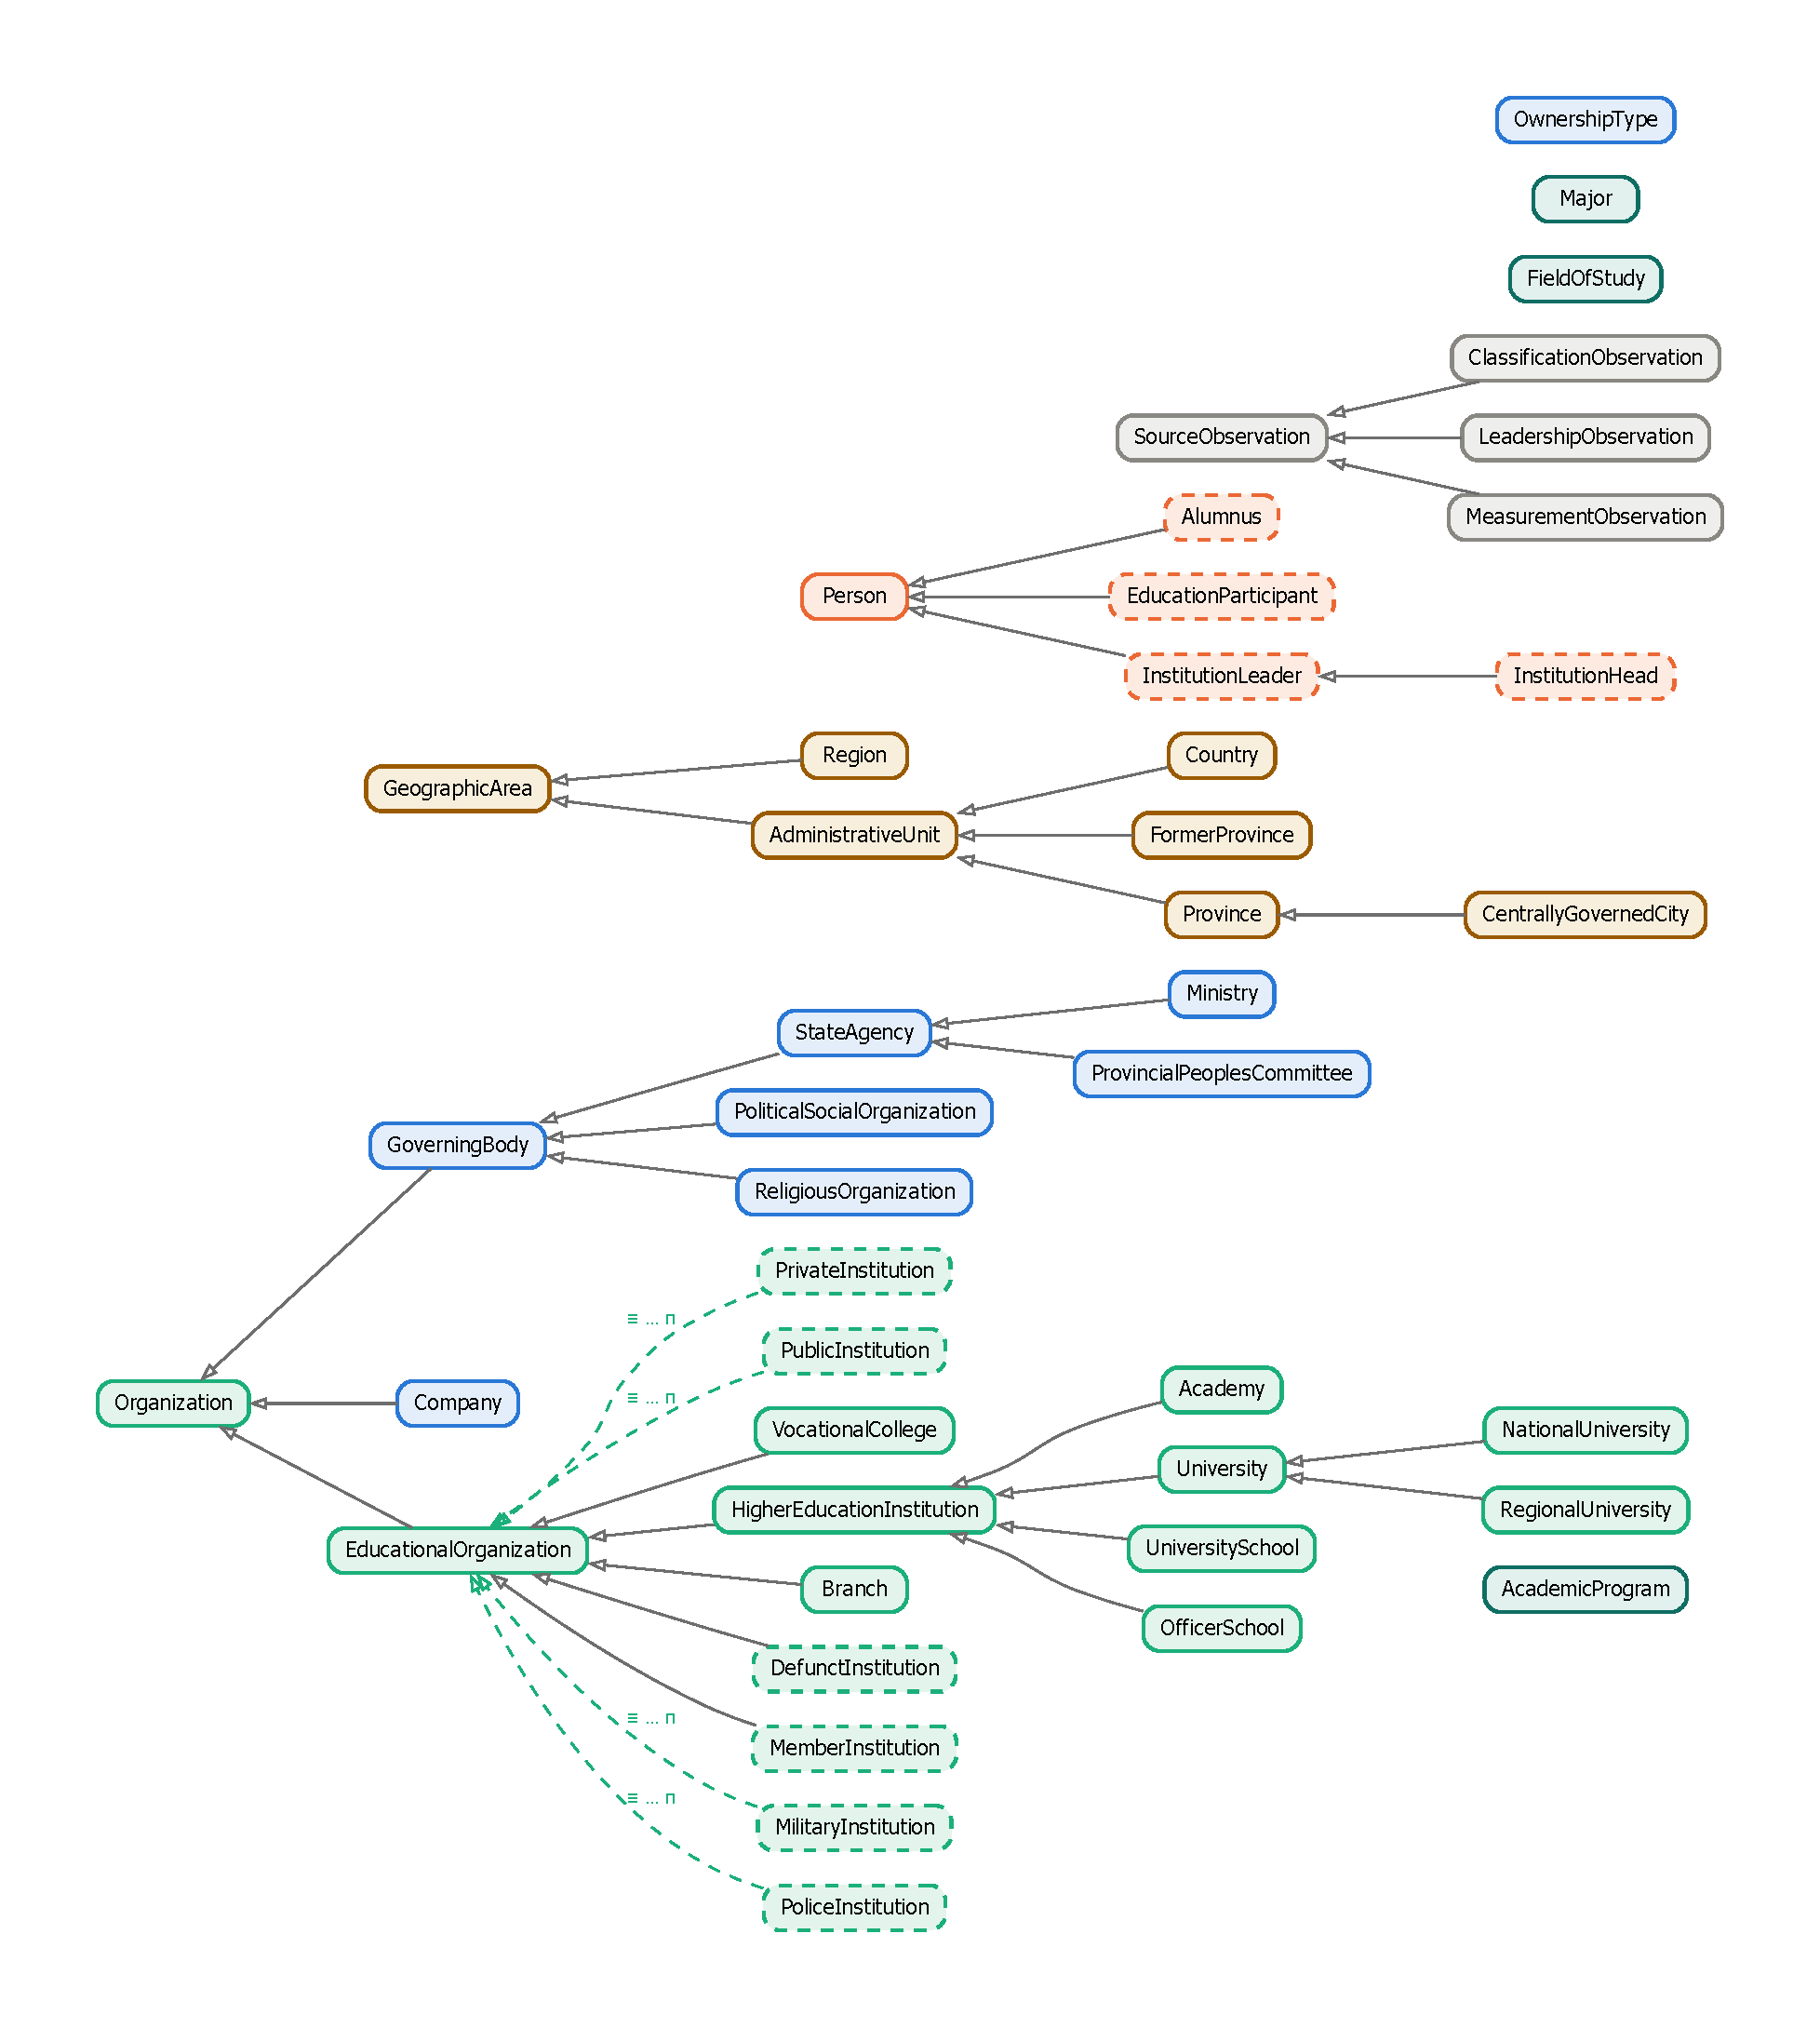
\includegraphics[height=0.9\textheight,width=\textwidth,keepaspectratio]{figures/gen/ontology-hierarchy.pdf}
\caption{Phân cấp lớp của ontology \texttt{vnedu:} 2.4 (sinh tự động từ \texttt{ontology/vnedu.ttl}). Mũi tên rỗng:
\texttt{rdfs:subClassOf}; viền đứt: lớp định nghĩa bằng \texttt{owl:equivalentClass} (nhãn ``\(\equiv\dots\sqcap\)'').
Màu biểu thị mô-đun.}\label{fig:hierarchy}
\end{figure}

\subsection{Thuộc tính và quan hệ}
\Cref{fig:relations} biểu diễn các quan hệ chính giữa các lớp: mỗi cạnh liền là một thuộc tính đối tượng, đi từ miền
tới miền giá trị. Để hình dễ đọc, các thuộc tính nghịch đảo (ví dụ \vn{hasAlumnus}) và thuộc tính con (ví dụ
\vn{rector} \(\sqsubseteq\) \vn{hasHead}) được ẩn. Danh sách đầy đủ \metricObjectProperties{} thuộc tính đối tượng và
\metricDataProperties{} thuộc tính dữ liệu nằm ở \cref{tab:props} (\cref{app:properties}).

\begin{figure}[htbp]
\centering
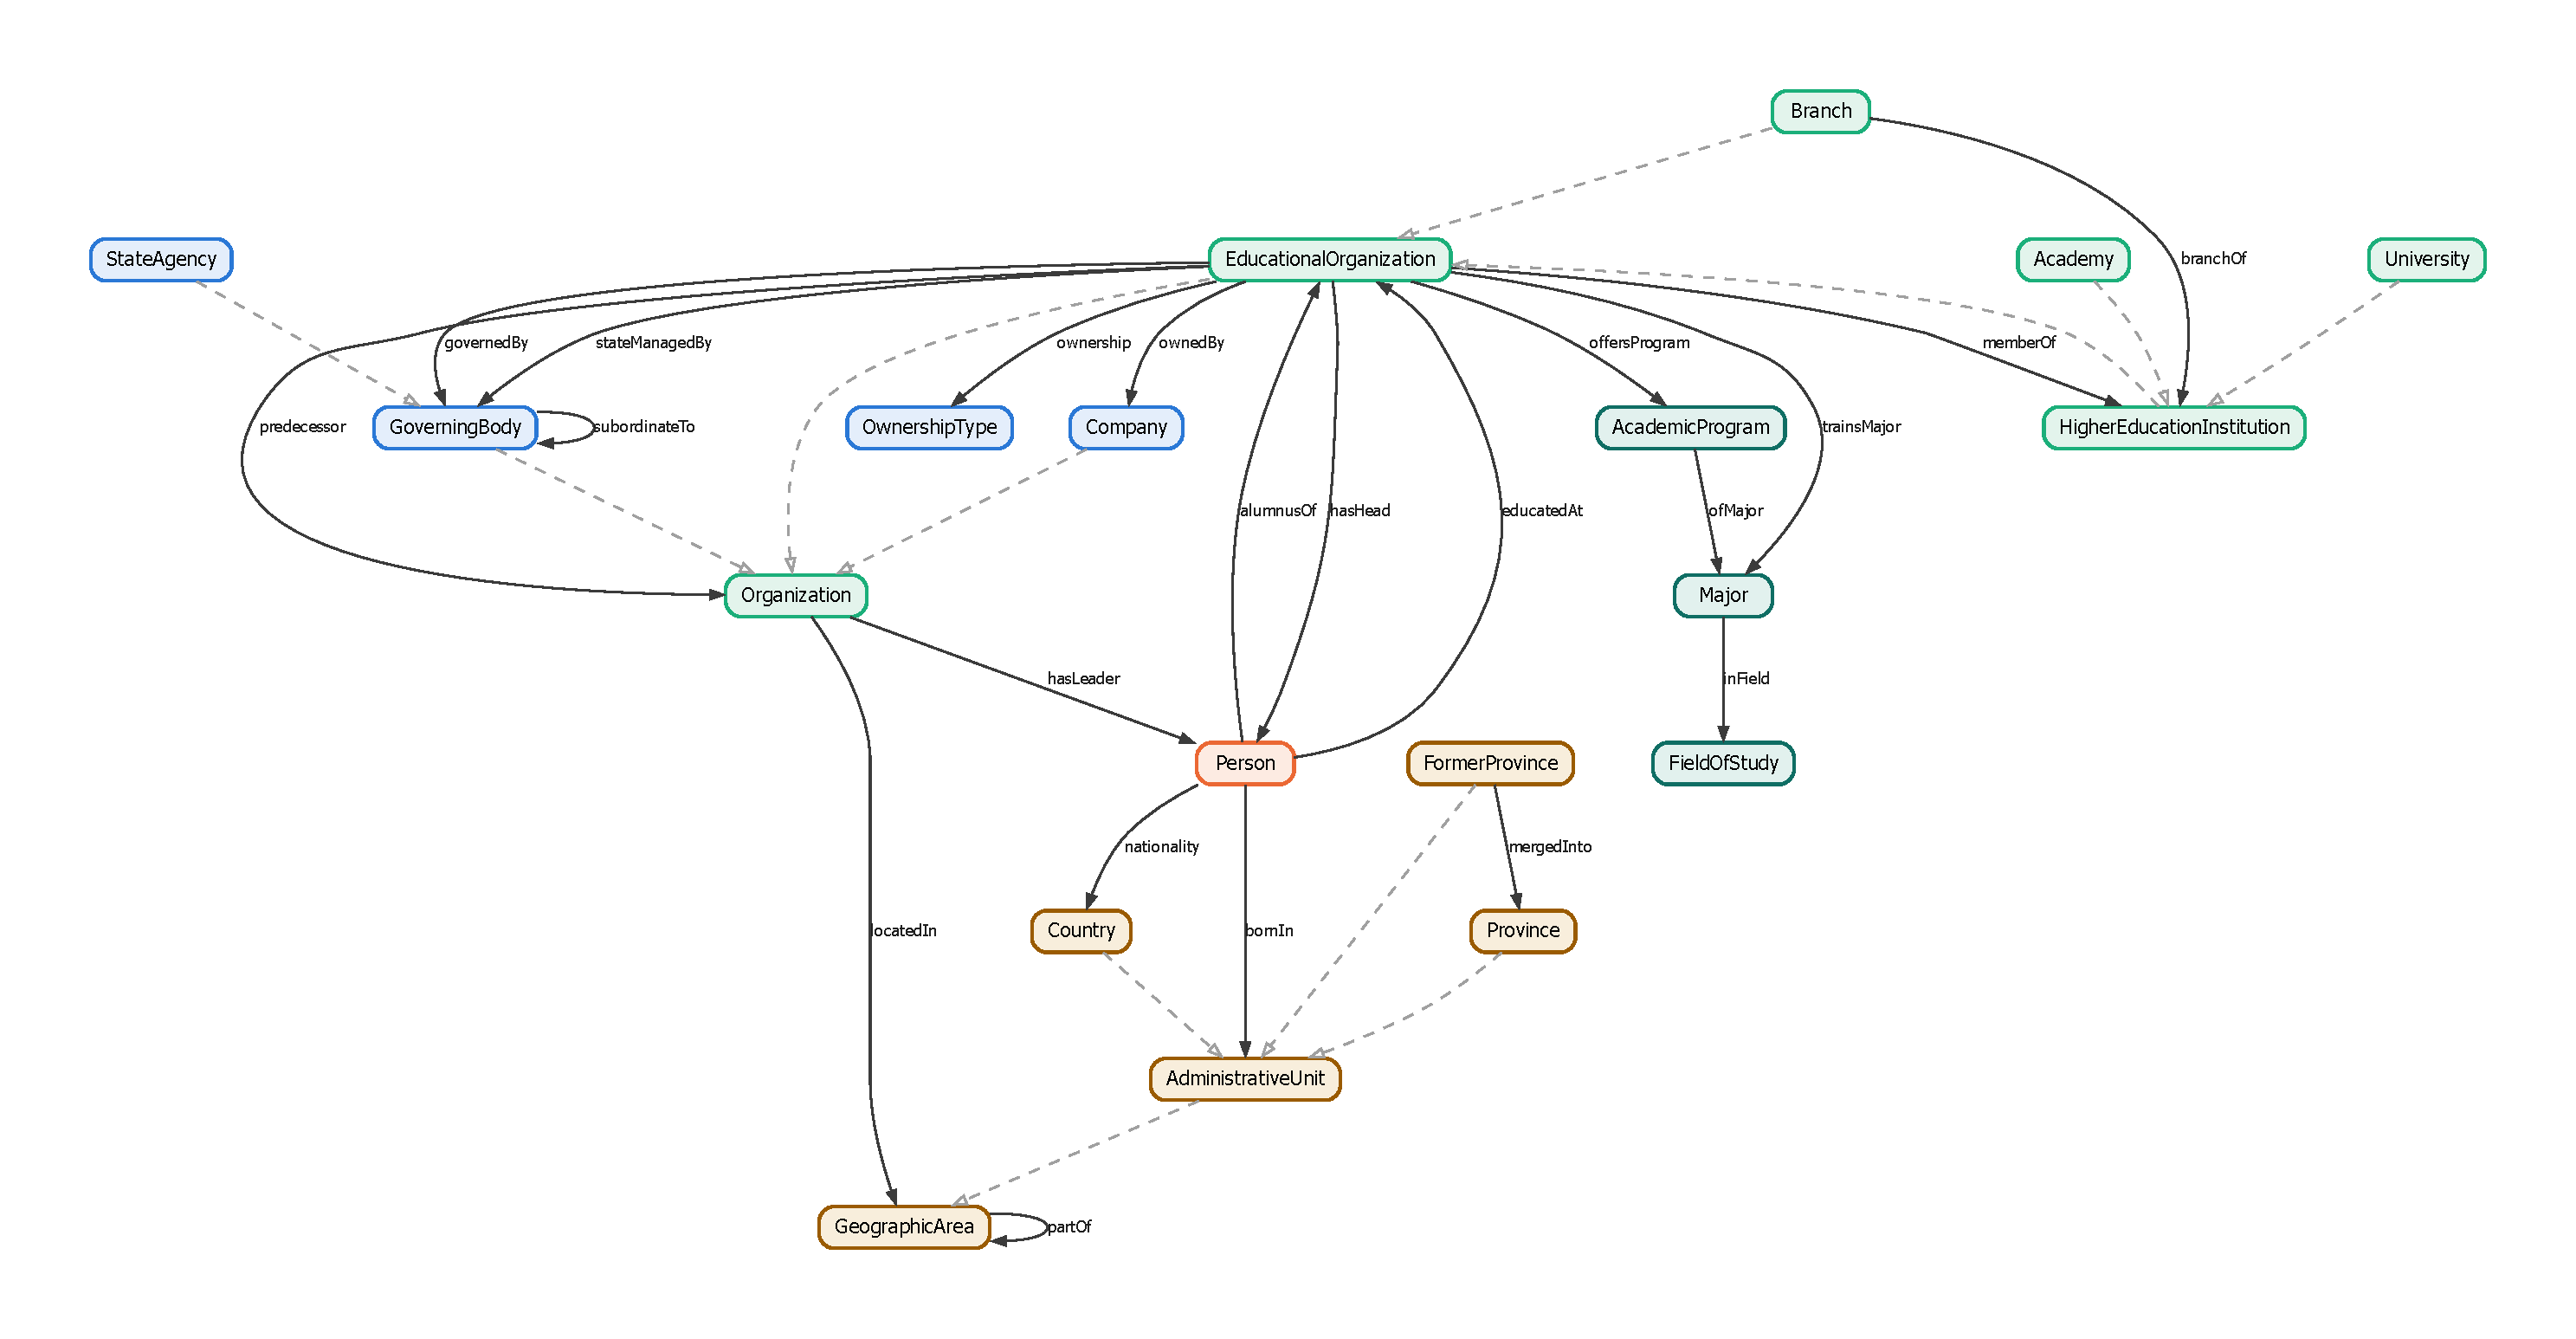
\includegraphics[width=\textwidth]{figures/gen/ontology-relations.pdf}
\caption{Bản đồ quan hệ giữa các lớp. Cạnh liền có nhãn: thuộc tính đối tượng (miền \(\to\) miền giá trị); cạnh đứt
mũi tên rỗng: \texttt{rdfs:subClassOf}.}\label{fig:relations}
\end{figure}

\subsection{Tiên đề và ngữ nghĩa}\label{sec:axioms}
Ngoài phân cấp, ontology dùng các cấu trúc OWL~2~RL sau để mã hoá tri thức miền.

\paragraph{Lớp định nghĩa bằng hạn chế giá trị.} Một cơ sở là \emph{cơ sở quân đội} khi và chỉ khi nó do Bộ Quốc phòng
quản lý. Tương tự cho công an, công lập và tư thục:
\codetitle{Lớp định nghĩa (trích \texttt{ontology/vnedu.ttl})}
\begin{code}
vnedu:MilitaryInstitution owl:equivalentClass [ owl:intersectionOf ( vnedu:EducationalOrganization
    [ a owl:Restriction ; owl:onProperty vnedu:governedBy ; owl:hasValue vnedu:MinistryOfNationalDefence ] ) ] .
vnedu:PrivateInstitution owl:equivalentClass [ owl:intersectionOf ( vnedu:EducationalOrganization
    [ a owl:Restriction ; owl:onProperty vnedu:ownership ; owl:hasValue vnedu:PrivateOwnership ] ) ] ;
    owl:disjointWith vnedu:PublicInstitution .
\end{code}

\paragraph{Chuỗi thuộc tính.} Chuỗi thuộc tính (\texttt{owl:propertyChainAxiom}) cho phép suy ra quan hệ bắc cầu qua
các loại quan hệ khác nhau:
\begin{align*}
\textit{locatedIn} \circ \textit{partOf} &\sqsubseteq \textit{locatedIn} && \text{(trường ở Hà Nội thì ở Bắc Bộ)}\\
\textit{locatedIn} \circ \textit{mergedInto} &\sqsubseteq \textit{locatedIn} && \text{(trường ở tỉnh cũ thì ở tỉnh mới)}\\
\textit{governedBy} \circ \textit{subordinateTo} &\sqsubseteq \textit{governedBy} && \text{(Học viện thuộc Tổng cục
\(\to\) thuộc Bộ)}\\
\textit{offersProgram} \circ \textit{ofMajor} &\sqsubseteq \textit{trainsMajor} && \text{(có chương trình ngành X
\(\to\) đào tạo X)}
\end{align*}
Nhờ chuỗi thứ hai, câu hỏi \CQ{1} trả lời được theo 34 tỉnh mới dù nguồn ghi địa chỉ theo 63 tỉnh cũ. Nhờ chuỗi thứ
ba, một trường do Tổng cục Chính trị (thuộc Bộ Quốc phòng) quản lý vẫn được phân loại là \vn{MilitaryInstitution}.

\paragraph{Lớp định nghĩa bằng lượng từ tồn tại.} Người đứng đầu ít nhất một cơ sở giáo dục được phân loại là
\vn{InstitutionHead}:
\(\textit{Person} \sqcap \exists\,\textit{headOf}.\textit{EducationalOrganization} \sqsubseteq
\textit{InstitutionHead}\). Đây là dạng tiên đề được phép trong OWL~2~RL vì lượng từ tồn tại nằm ở \emph{vế trái}.

\paragraph{Thuộc tính nghịch đảo và thuộc tính hàm.} Ontology có các cặp nghịch đảo (\texttt{owl:inverseOf}), ví dụ
\vn{governs}~\(\equiv\) \vn{governedBy}\(^{-}\). \vn{foundingYear} là thuộc tính hàm (mỗi cơ sở chỉ có một năm thành
lập), nên khi hai nguồn mâu thuẫn, pipeline phải chọn một giá trị và ghi giá trị còn lại vào một quan sát.

\paragraph{Ràng buộc rời nhau.} \texttt{owl:AllDisjointClasses} được khai báo cho ba nhóm: các loại hình cơ sở GDĐH
(\vn{University}, \vn{UniversitySchool}, \vn{Academy}, \vn{OfficerSchool}); \vn{HigherEducationInstitution},
\vn{Branch} và \vn{VocationalCollege}; các loại cơ quan chủ quản (\vn{StateAgency},
\vn{PoliticalSocialOrganization}, \vn{ReligiousOrganization}). Ngoài ra, \vn{PublicInstitution} rời
\vn{PrivateInstitution}. Các ràng buộc này giúp phát hiện lỗi dữ liệu, chẳng hạn một cơ sở vừa được nguồn này ghi là
công lập, vừa được nguồn khác ghi là tư thục.

\subsection{Mô hình hoá nguồn gốc và thời gian: \texttt{SourceObservation}}
Wikipedia ghi ``Hiệu trưởng: Nguyễn Văn A'' nhưng không cho biết từ khi nào và đến khi nào. Nếu chuyển thẳng thành
triple \texttt{trường vnedu:rector người}, đồ thị sẽ khẳng định một điều có thể đã sai. Chúng tôi dùng mẫu
\emph{reification có kiểu}: mỗi khẳng định phụ thuộc thời gian được ghi thành một cá thể \vn{SourceObservation}
(\texttt{prov:Entity}) có nguồn, thời điểm chụp (\vn{snapshotDigest}), trạng thái thời gian (\vn{temporalStatus}) và
khoảng hiệu lực (\vn{validFrom}, \vn{validThrough}) nếu biết. Quan sát tự nó không khẳng định nội dung
(reification không kéo theo triple gốc), nên đồ thị không ngầm tuyên bố một người \emph{đang} giữ chức vụ. Đồ thị hiện có \metricObservations{} quan sát, chiếm khoảng 35{,}5 nghìn triple siêu dữ liệu.

URI của quan sát là băm SHA-256 của nội dung (chủ thể, vị từ, giá trị, nguồn, khoảng hiệu lực), nên quan sát giống
nhau luôn có cùng URI qua các lần chạy. Trong \metricObservations{} quan sát, 46 quan sát có thông tin thời gian
(\texttt{"qualified"}); số còn lại mang trạng thái \texttt{"unknown"}, tức nguồn không cho biết thời điểm hiệu lực.

\codetitle{Một quan sát lãnh đạo thật trong đồ thị (rút gọn URI)}
\begin{code}
<.../resource/observation/bf26547025b8…6e84>
    a vnedu:SourceObservation , vnedu:LeadershipObservation ;
    rdf:subject   university:truong-dai-hoc-van-hoa-thanh-pho-ho-chi-minh ;
    rdf:predicate vnedu:councilChair ;
    rdf:object    person:trinh-dang-khoa ;
    prov:wasDerivedFrom wd:Q5873981 , <https://vi.wikipedia.org/w/index.php?oldid=75085609> ;
    vnedu:snapshotDigest "bf26547025b8a71a82742f3dc9a912d9e57b58edc3df0b31b80e18aab7fa6e84" ;
    vnedu:temporalStatus "unknown" .
\end{code}

\subsection{Căn chỉnh với từ vựng ngoài}
Để dữ liệu dễ dùng với công cụ hiện có, 26 lớp/thuộc tính được căn chỉnh (\texttt{rdfs:subClassOf},
\texttt{rdfs:subPropertyOf}, \texttt{owl:equivalentClass}) với schema.org~\cite{guha2016schemaorg} (ví dụ
\vn{HigherEducationInstitution} \(\sqsubseteq\) \texttt{schema:CollegeOrUniversity}), DBpedia (\texttt{dbo:University}),
FOAF (\texttt{foaf:Person}), PROV-O và SKOS. Căn chỉnh chỉ theo hướng \emph{con của} ở những chỗ ngữ nghĩa không trùng
hoàn toàn, để tránh kéo theo các hệ quả không mong muốn. Chúng tôi kiểm tra điều này bằng cách nạp TBox DBpedia
(34{,}544 triple) cùng ontology vào HermiT, và kết quả vẫn nhất quán (\cref{sec:reason}).

\subsection{Một ví dụ cá thể: Đại học Bách khoa Hà Nội}
\Cref{fig:abox} minh hoạ lân cận của cá thể \texttt{university/dai-hoc-bach-khoa-ha-noi} trong ABox và liên hệ tới TBox.
Đoạn Turtle dưới đây là mô tả thật trong đồ thị (đã lược bớt):

\codetitle{Mô tả RDF của HUST (trích \texttt{vnedu-data.ttl} và \texttt{vnedu-links.ttl})}
\begin{code}
university:dai-hoc-bach-khoa-ha-noi a vnedu:University ;
    rdfs:label "Đại học Bách khoa Hà Nội"@vi , "Hanoi University of Science and Technology"@en ;
    vnedu:shortName "HUST" , "BKHN" ;          vnedu:admissionCode "BKA" ;
    vnedu:foundingYear 1956 ;                  vnedu:establishmentYear 1956 ;
    vnedu:ownership vnedu:PublicOwnership ;
    vnedu:directlyGovernedBy organization:bo-giao-duc-va-dao-tao ;   # QĐ 1723/QĐ-TTg
    vnedu:locatedIn province:ha-noi ;           vnedu:website <https://hust.edu.vn/> ;
    geo:lat 21.006389 ; geo:long 105.843056 ;
    prov:wasDerivedFrom wd:Q3075696 , <https://tuyensinh.moet.gov.vn/ts/> ,
        <https://congbao.chinhphu.vn/van-ban/quyet-dinh-so-1723-qd-ttg-45825/58191.htm> ;
    owl:sameAs wd:Q3075696 , dbr:Hanoi_University_of_Science_and_Technology ,
        <https://ror.org/04nyv3z04> ;
    foaf:isPrimaryTopicOf <https://vi.wikipedia.org/wiki/Đại_học_Bách_khoa_Hà_Nội> .
\end{code}

\begin{figure}[htbp]
\centering
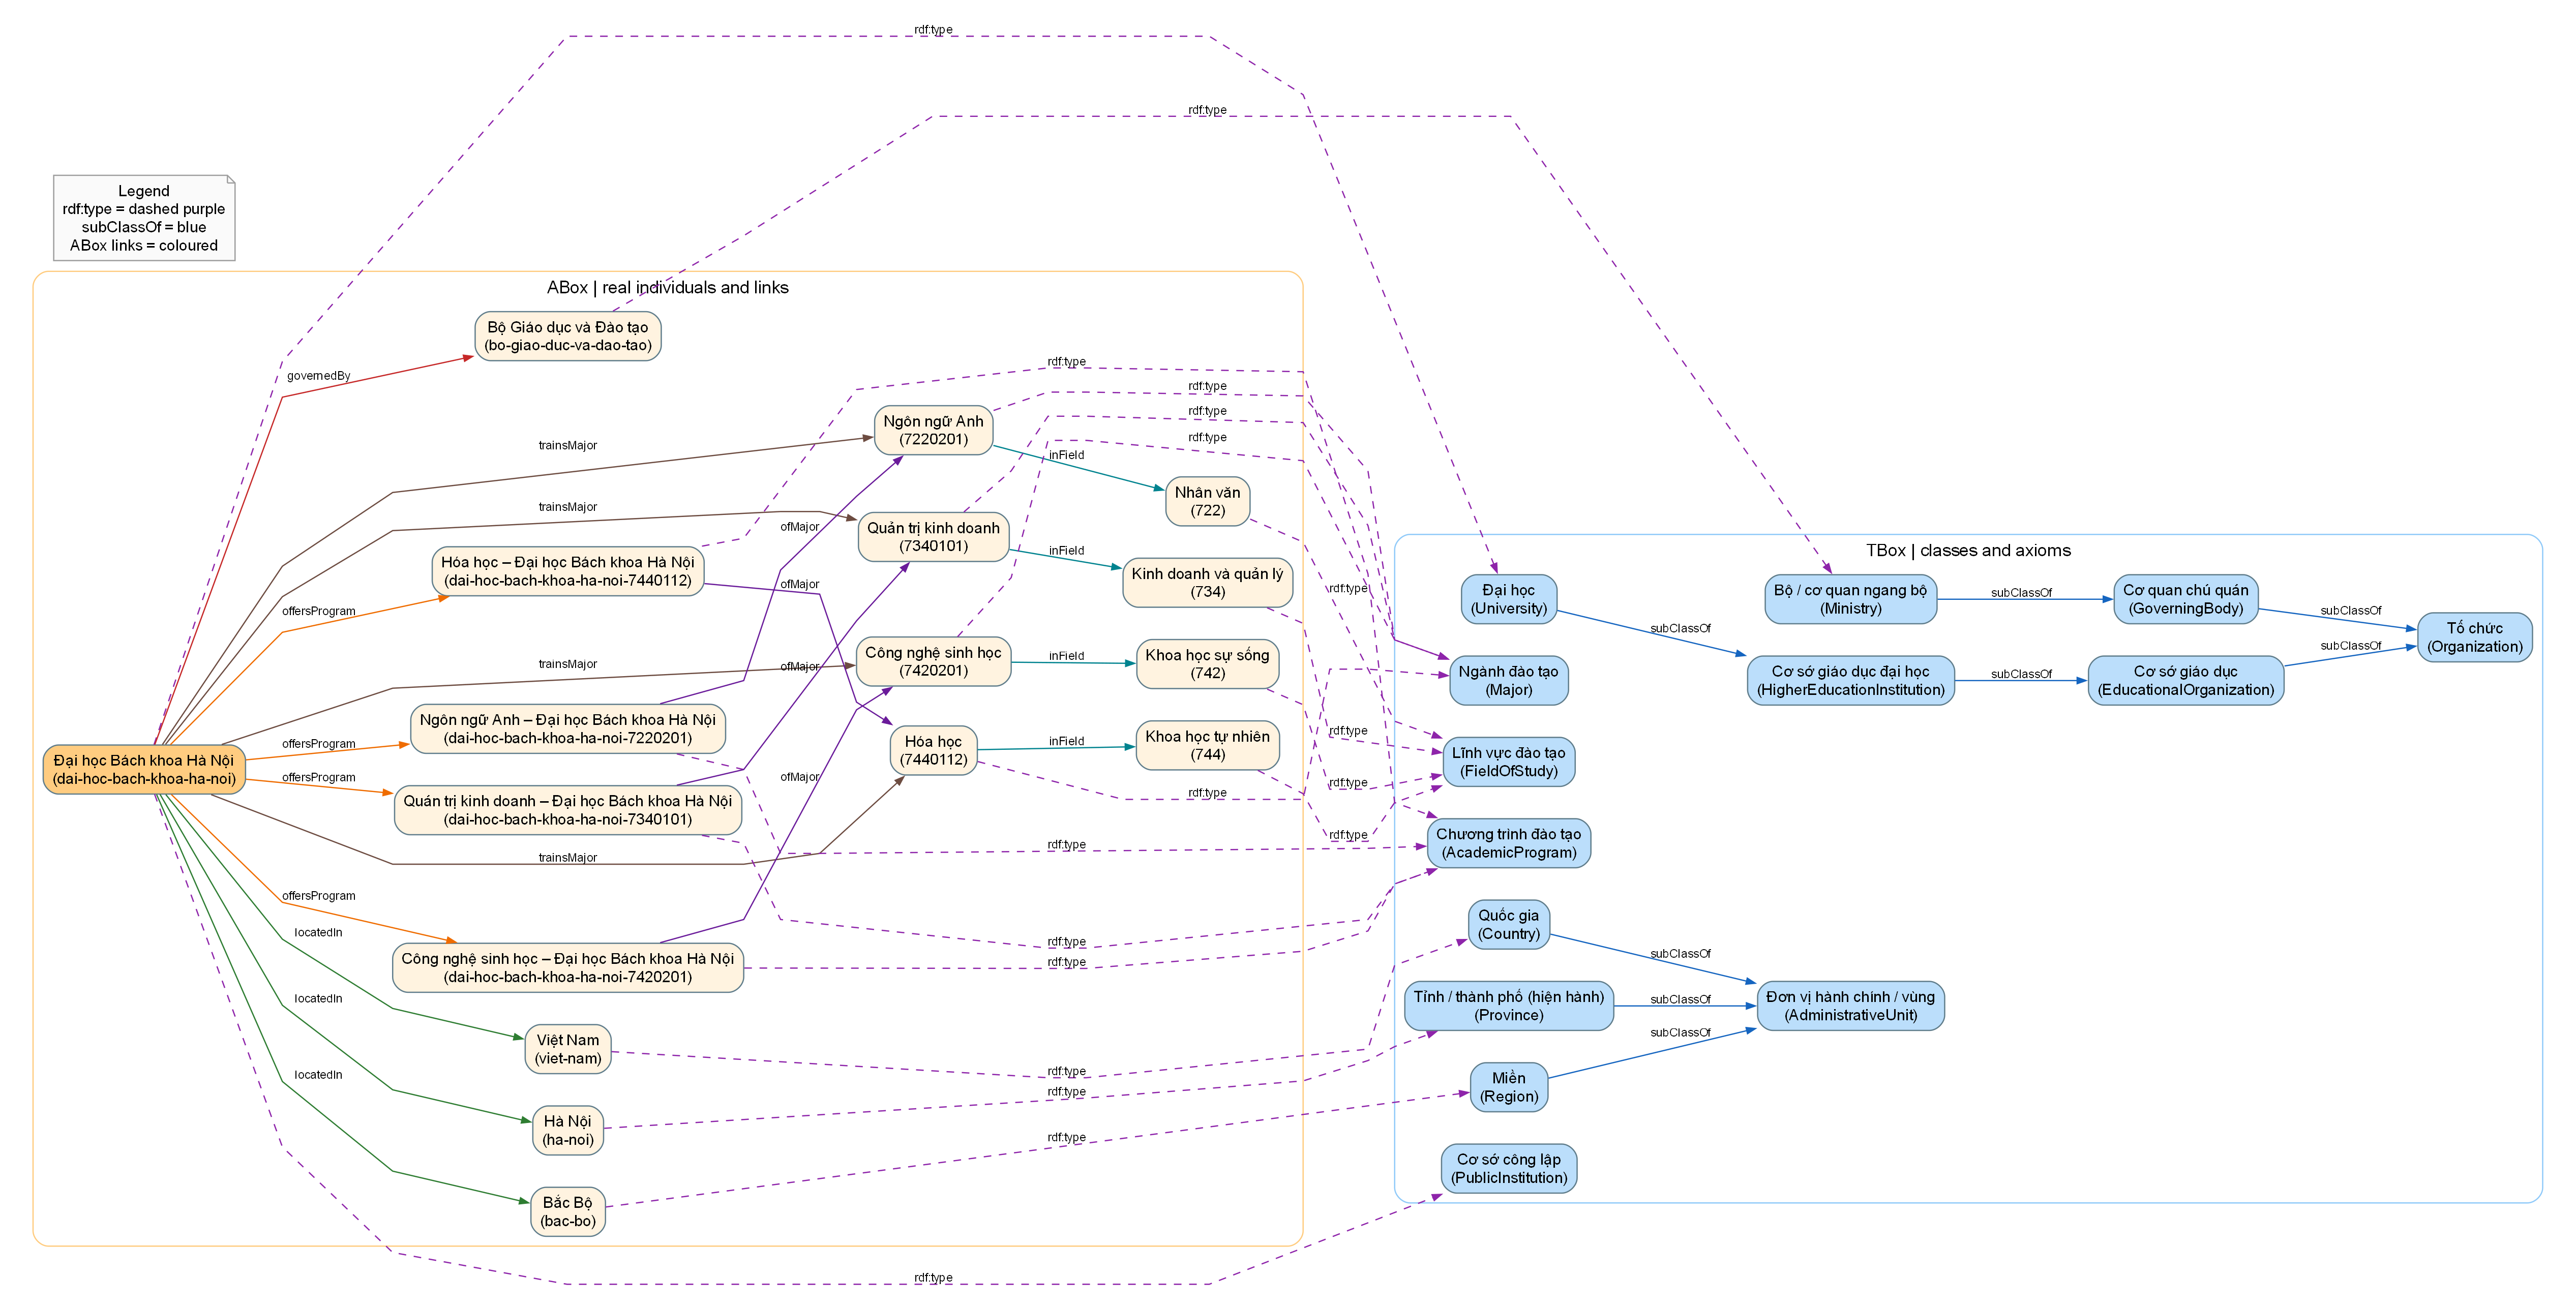
\includegraphics[width=\textwidth]{figures/abox-instance-neighborhood.png}
\caption{Lân cận ABox của Đại học Bách khoa Hà Nội (trái) và các lớp TBox tương ứng (phải). Nét đứt tím:
\texttt{rdf:type}; xanh: \texttt{rdfs:subClassOf}; các màu khác: quan hệ giữa cá thể.}\label{fig:abox}
\end{figure}

% ================================================================= 6. XÂY DỰNG DỮ LIỆU
\section{Xây dựng dữ liệu và liên kết}\label{sec:data}

\subsection{Thu thập có bộ đệm (Bronze)}
Mọi yêu cầu HTTP đi qua mô-đun \texttt{httpcache}. Khoá của bộ đệm là phương thức, URL và thân yêu cầu đã chuẩn hoá.
Các phản hồi được đóng gói thành \texttt{data/bronze/http\_cache.zip} và đưa vào kho mã. Cách làm này có ba lợi ích:
(i) pipeline xây lại được ngoại tuyến; (ii) có thể kiểm tra lại đúng dữ liệu đã dùng (Wikipedia được gọi kèm
\texttt{oldid} của phiên bản bài); (iii) tránh gửi tải lặp lại tới WDQS.

\subsection{Tích hợp và giải quyết xung đột (Silver)}
\paragraph{So khớp thực thể.} Một cơ sở được nhận diện qua QID Wikidata, mã tuyển sinh MOET, và tên đã chuẩn hoá (bỏ
dấu, bỏ tiền tố ``Trường'', thống nhất ``Đại học''/``ĐH''). Các cặp không tự khớp được ghi vào bảng đối chiếu thủ công
có trích nguồn.

\paragraph{Thứ tự ưu tiên nguồn.} Với mỗi trường dữ liệu, các nguồn được ưu tiên theo mức độ chính thức: văn bản pháp
lý \(>\) MOET \(>\) Wikidata \(>\) Wikipedia \(>\) DBpedia. Giá trị bị loại không bị xoá mà được ghi thành
\vn{ClassificationObservation} hoặc \vn{MeasurementObservation}, nên người dùng vẫn thấy được mâu thuẫn.

\paragraph{Quy đổi địa giới.} Bảng \texttt{province\_mergers\_2025.csv} ánh xạ 63 tỉnh cũ sang 34 tỉnh mới theo
NQ~202/2025/QH15. Tỉnh cũ được mô hình hoá là \vn{FormerProvince} có \vn{mergedInto}. Nhờ chuỗi thuộc tính, bộ suy
luận tự quy đổi; dữ liệu gốc không bị sửa.

\paragraph{Chủ quản trực tiếp.} \vn{directlyGovernedBy} chỉ được gán khi có văn bản pháp lý (ví dụ QĐ~1723/QĐ-TTg chuyển
ĐHBK Hà Nội thành đại học trực thuộc Bộ GD\&ĐT). Thông tin chủ quản do Wikidata/Wikipedia ghi nhận được giữ ở
\vn{reportedGovernedBy}. Hai thuộc tính này đều là thuộc tính con của \vn{governedBy}. Trong dữ liệu, cả 155/155 khẳng
định ``chủ quản quản lý trường'' đều có thuộc tính nghịch đảo \vn{governs} nhất quán.

\subsection{Thiết kế URI}
URI tuân theo mẫu \texttt{\{base\}/resource/\{loại\}/\{slug\}}, trong đó \emph{slug} là tên tiếng Việt bỏ dấu, viết
thường, nối bằng gạch ngang (ví dụ \texttt{/resource/university/dai-hoc-bach-khoa-ha-noi}). URI ổn định qua các phiên
bản: ánh xạ \texttt{uri\_map.json} được lưu lại, và slug của thực thể cũ không bao giờ bị cấp lại cho thực thể khác.
URI \texttt{/resource/…} (không đuôi) định danh \emph{sự vật}. Các \emph{tài liệu} mô tả sự vật có URI riêng bằng
cách thêm đuôi: \texttt{….ttl} (Turtle) và \texttt{….jsonld} (JSON-LD). Cách tách này tương tự cách DBpedia tách
\texttt{/resource/} và \texttt{/data/}.

\subsection{Liên kết ra ngoài}
Bước 4 sinh các loại liên kết sau:
\begin{itemize}
  \item \texttt{owl:sameAs} sang \textbf{Wikidata} cho cơ sở, tỉnh, người, cơ quan, miền và quốc gia. QID lấy từ nguồn
  gốc của bản ghi, không phải từ tìm kiếm mờ. Riêng cơ quan và miền chưa có QID thì tìm bằng API Wikidata với điều kiện
  nhãn tiếng Việt khớp chính xác và mô tả không thuộc danh sách loại trừ (tên họ, tạp chí, phim\dots).
  \item \texttt{owl:sameAs} sang \textbf{DBpedia}: khám phá qua endpoint DBpedia bằng truy vấn
  \texttt{?d owl:sameAs wd:Q…}. Chỉ chấp nhận khi ánh xạ là một--một.
  \item \texttt{owl:sameAs} sang \textbf{ROR} (cơ sở) và \textbf{GeoNames} (tỉnh).
  \item \texttt{skos:closeMatch} cho ngành và lĩnh vực. Dùng \texttt{closeMatch} thay vì \texttt{sameAs} vì khái niệm
  ``ngành'' trong danh mục Việt Nam không trùng hoàn toàn với khái niệm học thuật trên Wikidata. Việc dùng
  \texttt{sameAs} sai chỗ là lỗi phổ biến đã được Halpin và cộng sự~\cite{halpin2010sameas} phân tích.
  \item \texttt{foaf:isPrimaryTopicOf} sang bài Wikipedia tiếng Việt và tiếng Anh.
\end{itemize}

\begin{figure}[htbp]
\centering
\begin{tikzpicture}
\begin{axis}[xbar, width=0.82\textwidth, height=5.6cm, bar width=11pt, xmin=0,
  symbolic y coords={GeoNames,ROR,DBpedia,Wikipedia,Wikidata}, ytick=data,
  nodes near coords, nodes near coords align={horizontal}, every node near coord/.append style={font=\small},
  xlabel={Số triple liên kết}, enlarge y limits=0.15, enlarge x limits={upper,value=0.15},
  axis lines*=left, xmajorgrids, grid style={black!10}]
\addplot[fill=s1!70, draw=s1] coordinates {(\stLinkGeoNames,GeoNames) (\stLinkROR,ROR) (\stLinkDBpedia,DBpedia)
  (\stLinkWikipedia,Wikipedia) (\stLinkWikidata,Wikidata)};
\end{axis}
\end{tikzpicture}
\caption{Số liên kết ra ngoài theo bộ dữ liệu đích. Wikidata gồm 1{,}850 \texttt{owl:sameAs} và 35
\texttt{skos:closeMatch}; DBpedia gồm 202 \texttt{sameAs} và 26 \texttt{closeMatch}.}\label{fig:links}
\end{figure}

\paragraph{Không suy luận trên \texttt{sameAs} ra ngoài.} Liên kết \texttt{owl:sameAs} ra ngoài được tách thành
tệp riêng và \emph{không} đưa vào bước suy luận. Nếu đưa vào, quy tắc \texttt{eq-rep} của OWL~2~RL sẽ nhân bản mọi
triple sang URI của Wikidata và DBpedia, làm đồ thị phình gấp nhiều lần mà không thêm tri thức.

\subsection{Siêu dữ liệu bộ dữ liệu (VoID/DCAT)}
\texttt{void.ttl} mô tả bộ dữ liệu bằng \texttt{void:Dataset} và \texttt{dcat:Dataset}: giấy phép, nhà xuất bản, số
triple/thực thể, endpoint SPARQL, \texttt{void:uriSpace}, các \texttt{void:Linkset} tới từng đích kèm số liên kết, và
\texttt{dct:modified} lấy theo thời điểm tất định của bản phát hành. VoID được sinh lại một cách idempotent: chạy bước
4 nhiều lần không làm tăng số đếm.

% ================================================================= 7. SUY LUẬN & KIỂM ĐỊNH
\section{Suy luận và kiểm định chất lượng}\label{sec:reason}

\subsection{Kiểm tra hồ sơ OWL và nhất quán}
\begin{enumerate}
  \item \textbf{Kiểm tra hồ sơ}: dùng bộ kiểm tra hồ sơ của OWL API~\cite{horridge2011owlapi}. Ontology (761 tiên đề)
  có \textbf{0 vi phạm} cả OWL~2~RL lẫn OWL~2~DL.
  \item \textbf{Bộ suy luận DL}: HermiT 1.4.3 trong Protégé 5.6~\cite{musen2015protege,glimm2014hermit} phân loại
  ontology. Kết quả: nhất quán, không có lớp không thoả mãn được, kể cả khi nạp thêm TBox DBpedia.
  \item \textbf{Kiểm tra nhất quán trên dữ liệu}: sau khi vật chất hoá, \texttt{step5\_reason.py} tìm cá thể thuộc hai
  lớp rời nhau, thuộc tính hàm có hai giá trị khác nhau, và cá thể thuộc \texttt{owl:Nothing}. Kết quả: 0 vi phạm.
\end{enumerate}

\subsection{Vật chất hoá suy luận OWL 2 RL}
owlrl áp dụng các luật OWL~2~RL trên hợp của ontology và dữ liệu (không gồm liên kết ra ngoài), sinh ra
\metricInferredTriples{} triple mới. Pipeline loại bỏ các kiểu tầm thường (\texttt{owl:Thing}, \texttt{rdfs:Resource}) và
ghi phần còn lại vào \texttt{vnedu-inferred.ttl}. Việc vật chất hoá giúp truy vấn ở phía phục vụ không cần bộ suy luận,
nên Oxigraph trong trình duyệt và rdflib trên Render đều trả kết quả suy luận. \Cref{tab:inferred} thống kê các lớp định
nghĩa được suy ra.

\begin{table}[htbp]
\centering\small
\caption{Phân loại tự động bằng lớp định nghĩa (không có cá thể nào được gán trực tiếp).}\label{tab:inferred}
\begin{tabular}{lrl}
\toprule
Lớp suy ra & Số cá thể & Tiên đề sử dụng \\
\midrule
\vn{PublicInstitution}   & 219 & \texttt{ownership} \(\ni\) \texttt{PublicOwnership} \\
\vn{PrivateInstitution}  &  35 & \texttt{ownership} \(\ni\) \texttt{PrivateOwnership} \\
\vn{MemberInstitution}   &  46 & \(\exists\,\texttt{memberOf}\) \\
\vn{MilitaryInstitution} &  21 & \texttt{governedBy} \(\ni\) Bộ Quốc phòng (qua chuỗi \texttt{subordinateTo}) \\
\vn{DefunctInstitution}  &  10 & \(\exists\,\texttt{dissolutionYear}\) \\
\vn{PoliceInstitution}   &   7 & \texttt{governedBy} \(\ni\) Bộ Công an \\
\vn{InstitutionHead}     & 198 & \(\exists\,\texttt{headOf}.\texttt{EducationalOrganization}\) \\
\bottomrule
\end{tabular}
\end{table}

\subsection{Kiểm định SHACL}
Tệp \texttt{shapes/vnedu-shapes.ttl} định nghĩa các hình dạng cho từng lớp chính. Ví dụ: \vn{admissionCode} phải khớp mẫu
ba chữ cái in hoa; \texttt{geo:lat}/\texttt{geo:long} phải nằm trong khung toạ độ của Việt Nam (vĩ độ 8--23,5; kinh độ
102--110); website phải là IRI \texttt{http(s)}; năm thành lập phải từ 1800 đến năm hiện tại và không sau năm giải thể
(ràng buộc SHACL-SPARQL); cơ sở tư thục không được có Bộ làm chủ quản; mỗi quan sát phải có đúng một
\vn{snapshotDigest} dạng SHA-256. Mức
nghiêm trọng được phân thành \texttt{Violation} (chặn công bố), \texttt{Warning} (thiếu dữ liệu không bắt buộc) và
\texttt{Info}. CI chặn bản phát hành nếu có vi phạm.

\begin{table}[htbp]
\centering\small
\caption{Kết quả kiểm định SHACL trên đồ thị đã suy luận.}\label{tab:shacl}
\begin{tabular}{lrl}
\toprule
Mức độ & Số kết quả & Nội dung \\
\midrule
Violation & \metricViolations{} & -- \\
Warning   & \metricWarnings{} & 21 cơ sở thiếu năm thành lập, 12 thiếu tỉnh \\
Info      & \metricInformationResults{} & một trường thành viên đặt ở tỉnh khác với đại học chủ quản \\
\bottomrule
\end{tabular}
\end{table}

% ================================================================= 8. CÔNG BỐ
\section{Công bố dữ liệu và ứng dụng}\label{sec:publish}

\subsection{URI tra cứu được và thương lượng nội dung}
Máy chủ trên Render thực hiện thương lượng nội dung theo tiêu đề \texttt{Accept} trên chính URI của sự vật:
\begin{itemize}
  \item \texttt{GET /resource/university/dai-hoc-bach-khoa-ha-noi} với \texttt{Accept: text/turtle},
  \texttt{application/ld+json}, \texttt{application/rdf+xml} hoặc \texttt{application/n-triples} trả về mô tả RDF; với
  \texttt{text/html} trả về trang infobox. Mọi phản hồi đều có \texttt{Vary: Accept} để bộ đệm trung gian không trộn
  lẫn các biểu diễn.
  \item Tài liệu RDF cũng truy cập được trực tiếp bằng đuôi \texttt{.ttl}/\texttt{.jsonld}, hoặc tham số
  \texttt{?format=}.
  \item Với SPARQL endpoint, định dạng kết quả không hỗ trợ (ví dụ \texttt{Accept: image/png}) nhận
  \texttt{406 Not Acceptable} kèm danh sách định dạng hỗ trợ.
\end{itemize}
Theo kết luận httpRange-14~\cite{w3c2005httprange14} và Cool URIs~\cite{w3c2008cooluris}, cách chuẩn mực nhất là
chuyển hướng \texttt{303} từ URI sự vật sang URI tài liệu. Chúng tôi chọn trả trực tiếp biểu diễn kèm \texttt{Vary}, đồng
thời công bố URI tài liệu riêng có đuôi. Lý do là GitHub Pages (kênh chính) không hỗ trợ 303, và cách làm này cho hai kênh
cùng một hành vi. Đây là một đánh đổi có chủ đích và được nêu ở \cref{sec:discussion}.
GitHub Pages không cho cấu hình chuyển hướng 303, nên trang tĩnh dùng giải pháp được W3C chấp
nhận~\cite{w3c2014bp}: mỗi trang HTML nhúng \texttt{<script type="application/ld+json">} và khai báo
\texttt{<link rel="alternate" type="text/turtle">} tới bản RDF tương ứng.

\begin{code}
$ curl -s -H "Accept: text/turtle" https://vnedu-lod.onrender.com/resource/university/dai-hoc-bach-khoa-ha-noi
$ curl -s https://pham-ng.github.io/Vietnam-University-Knowledge-Graph-ver2/resource/university/dai-hoc-bach-khoa-ha-noi.ttl
\end{code}

\subsection{SPARQL endpoint}
\texttt{/sparql} tuân thủ giao thức SPARQL 1.1: nhận \texttt{GET} và \texttt{POST}; trả kết quả dạng JSON, XML, CSV,
TSV cho \texttt{SELECT}/\texttt{ASK}, và Turtle, JSON-LD cho \texttt{CONSTRUCT}/\texttt{DESCRIBE}. Truy vấn liên hợp
\texttt{SERVICE} chỉ được gửi tới các endpoint trong danh sách cho phép (Wikidata, DBpedia). Công cụ dòng lệnh
\texttt{query.py} chạy được cả 19 truy vấn mẫu với đồ thị cục bộ hoặc với endpoint từ xa.

\subsection{Giao diện web}
Trang web (\cref{fig:web}) gồm các trang: trang chủ thống kê; tra cứu có bộ lọc; bản đồ cơ sở; trang ontology có sơ đồ
lớp tương tác; trang SPARQL có các truy vấn mẫu dạng ``chip'' bấm để chạy; và trang ``Liên kết LOD'' liệt kê các
linkset. Trên trang tĩnh, toàn bộ \metricUnionTriples{} triple (khoảng 5~MB) được nạp vào Oxigraph/WASM trong khoảng
0,24~giây, sau đó truy vấn chạy hoàn toàn trên máy người dùng. Mỗi trang tài nguyên có hộp thông tin (infobox) giống
Wikipedia, hiển thị chủ quản trực tiếp kèm số quyết định, lãnh đạo kèm nguồn, và các liên kết ra ngoài.

\begin{figure}[htbp]
\centering
\begin{subfigure}[t]{0.49\textwidth}\centering
  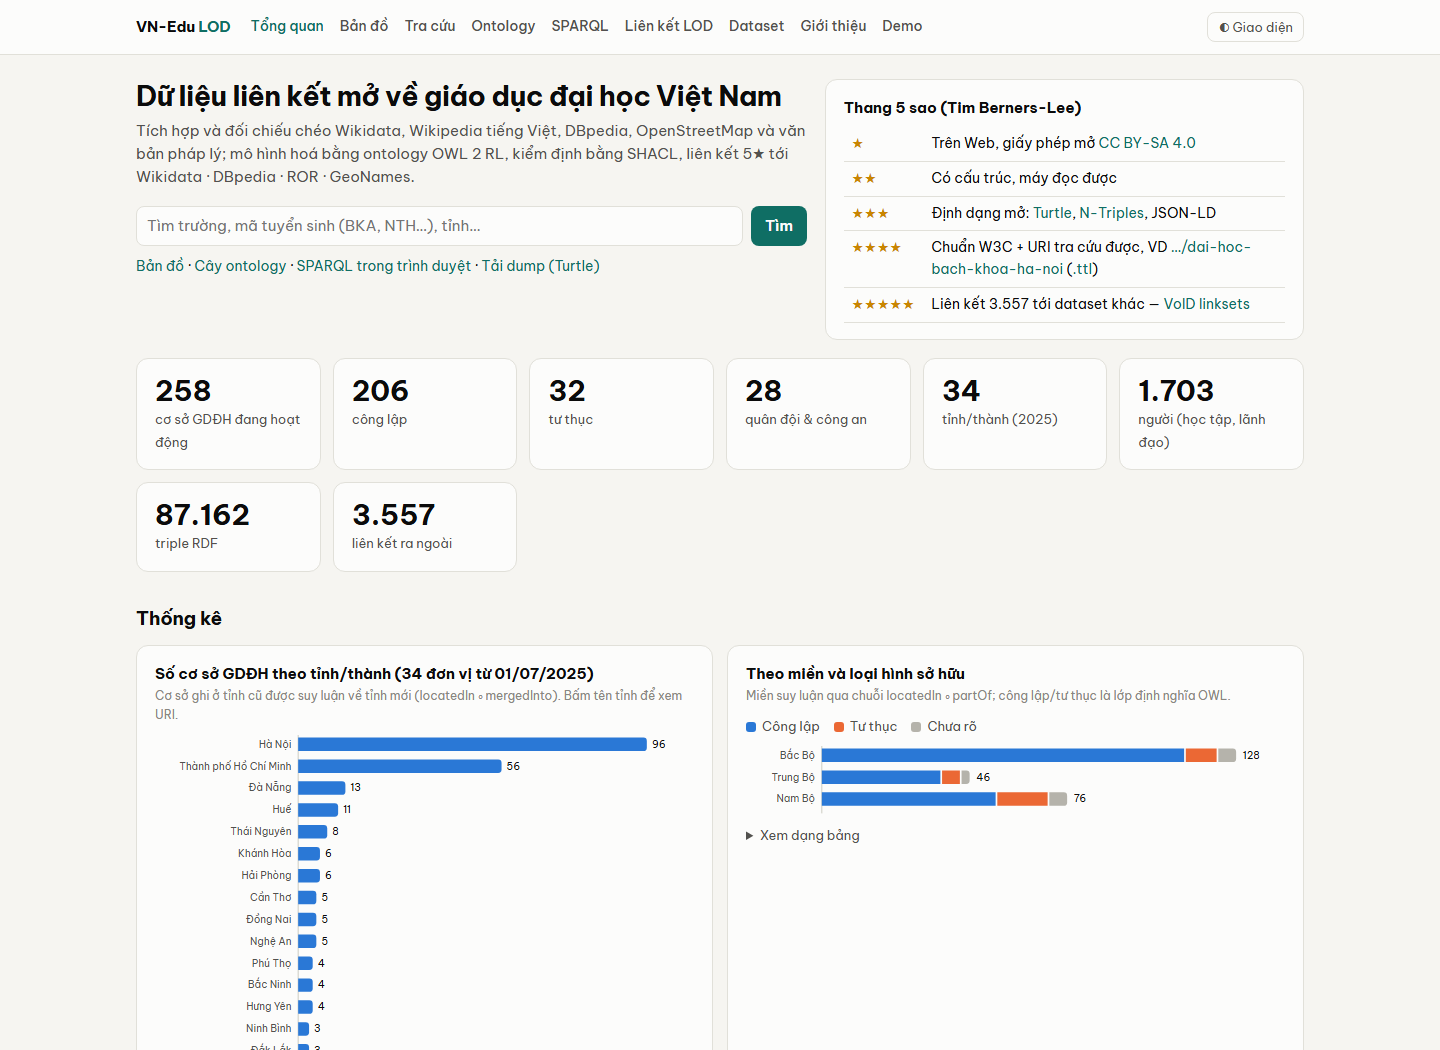
\includegraphics[width=\textwidth]{figures/gen/web-home.png}\caption{Trang chủ}\end{subfigure}\hfill
\begin{subfigure}[t]{0.49\textwidth}\centering
  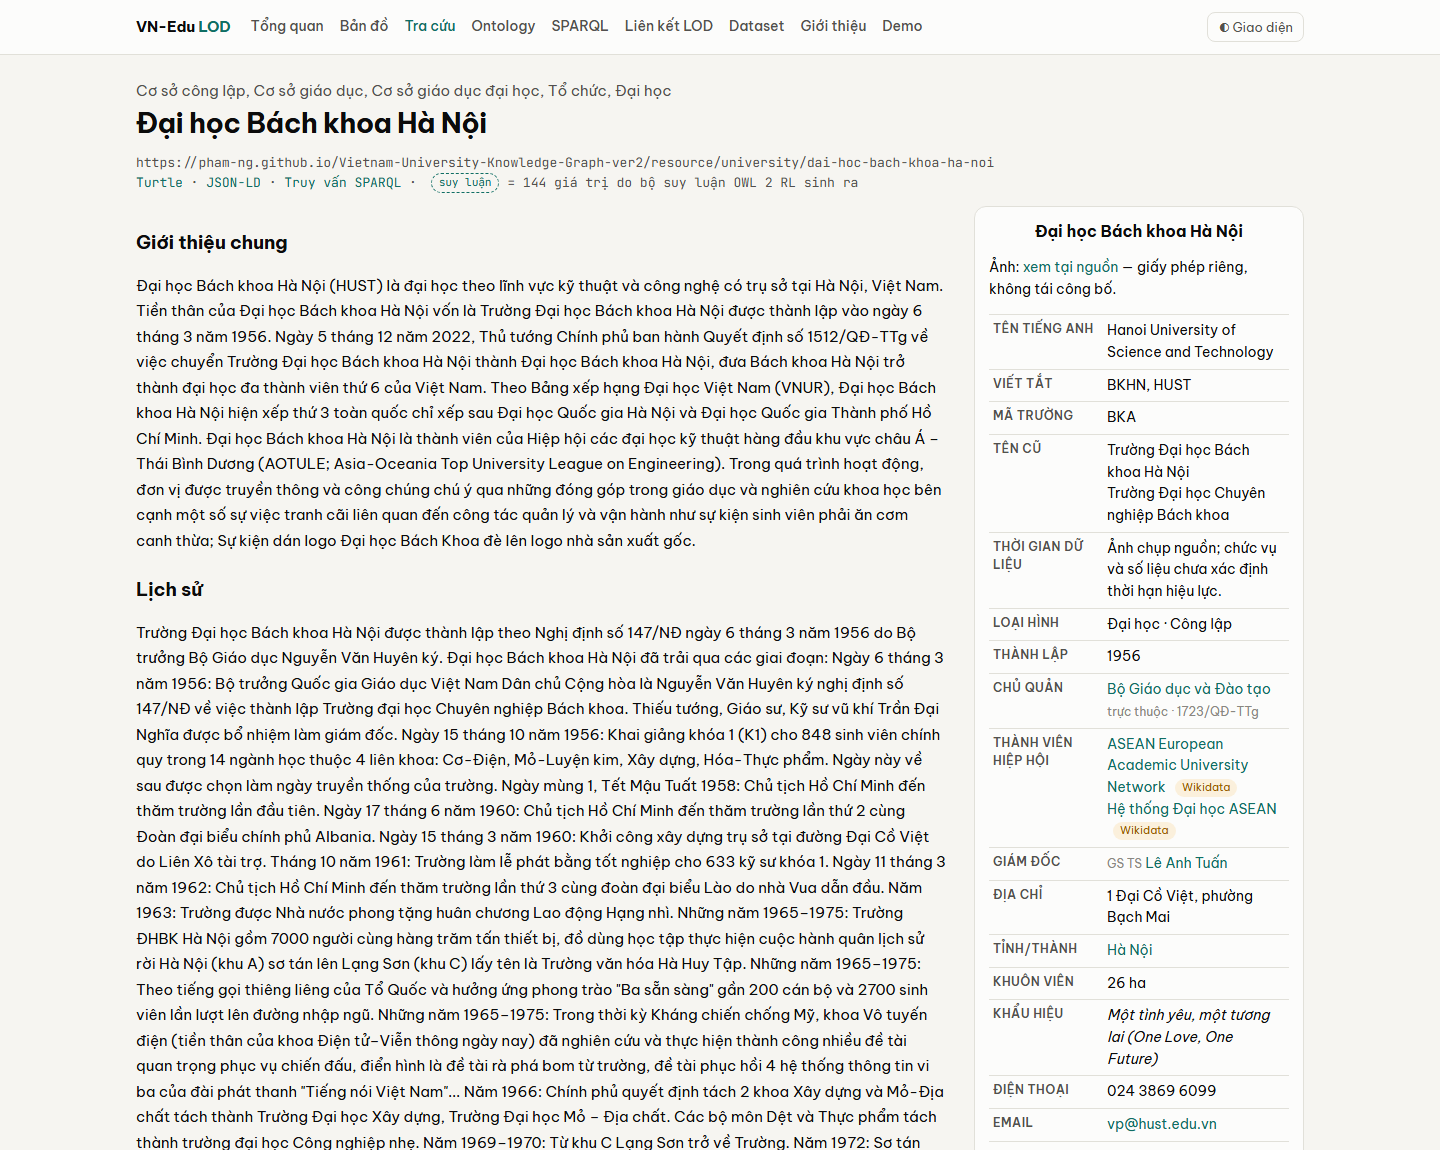
\includegraphics[width=\textwidth]{figures/gen/web-hust.png}\caption{Trang tài nguyên HUST}\end{subfigure}
\\[6pt]
\begin{subfigure}[t]{0.49\textwidth}\centering
  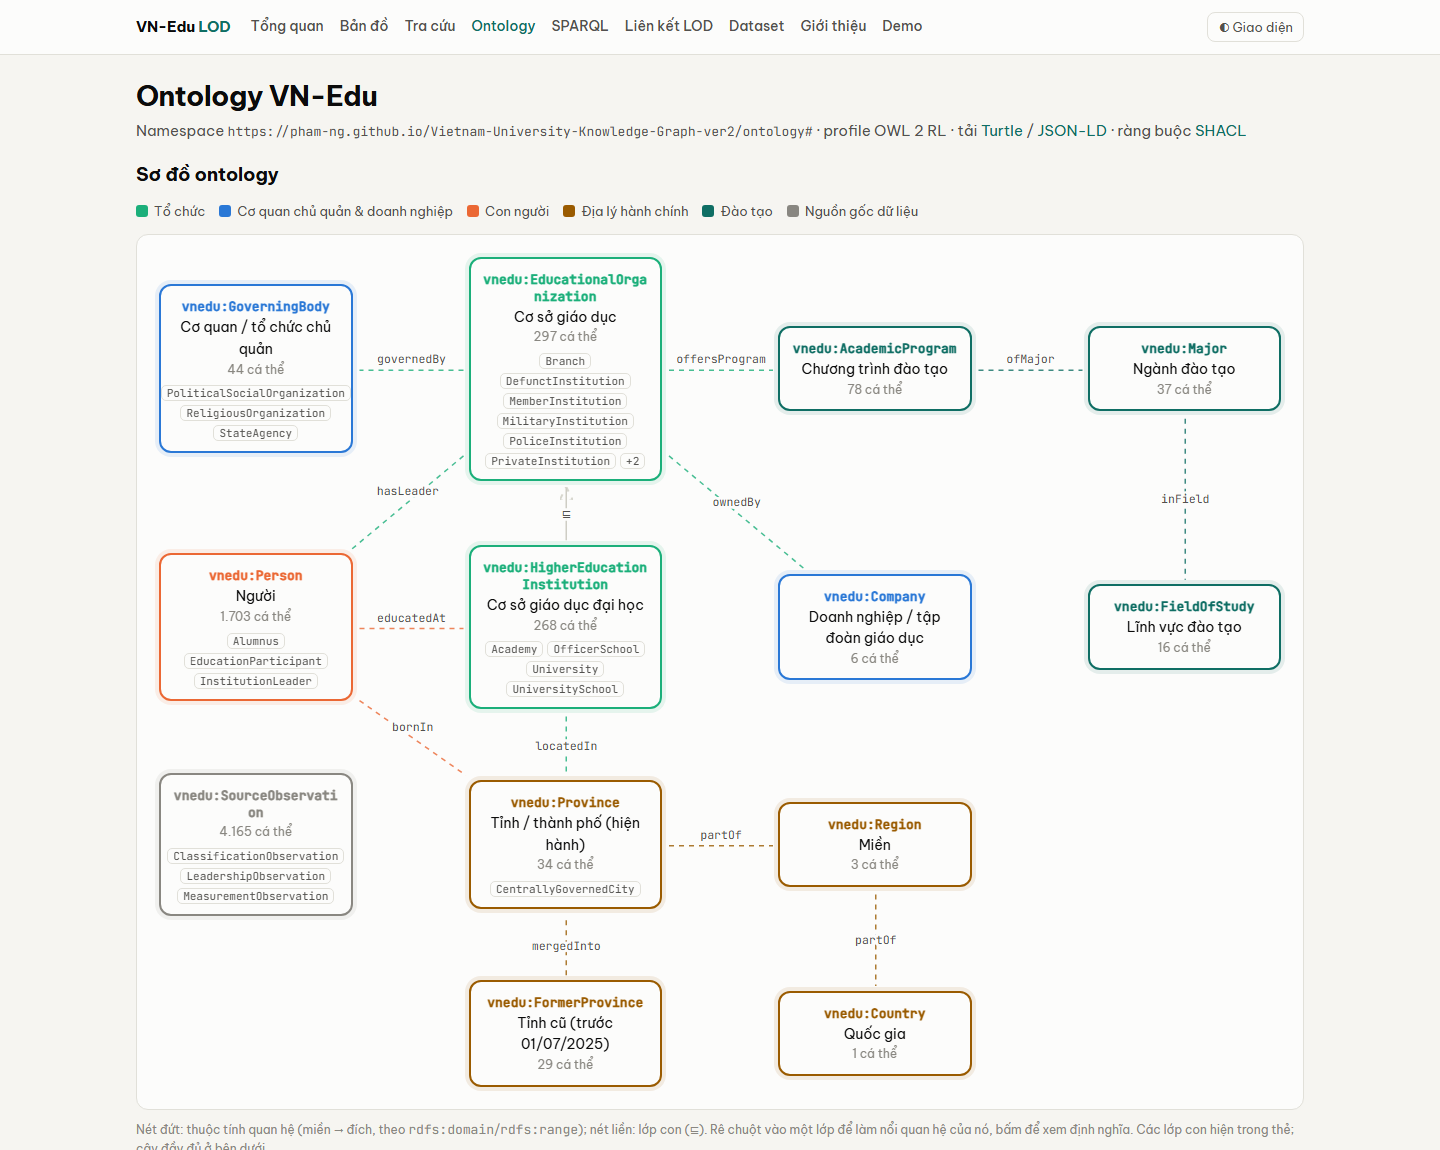
\includegraphics[width=\textwidth]{figures/gen/web-ontology.png}\caption{Sơ đồ ontology}\end{subfigure}\hfill
\begin{subfigure}[t]{0.49\textwidth}\centering
  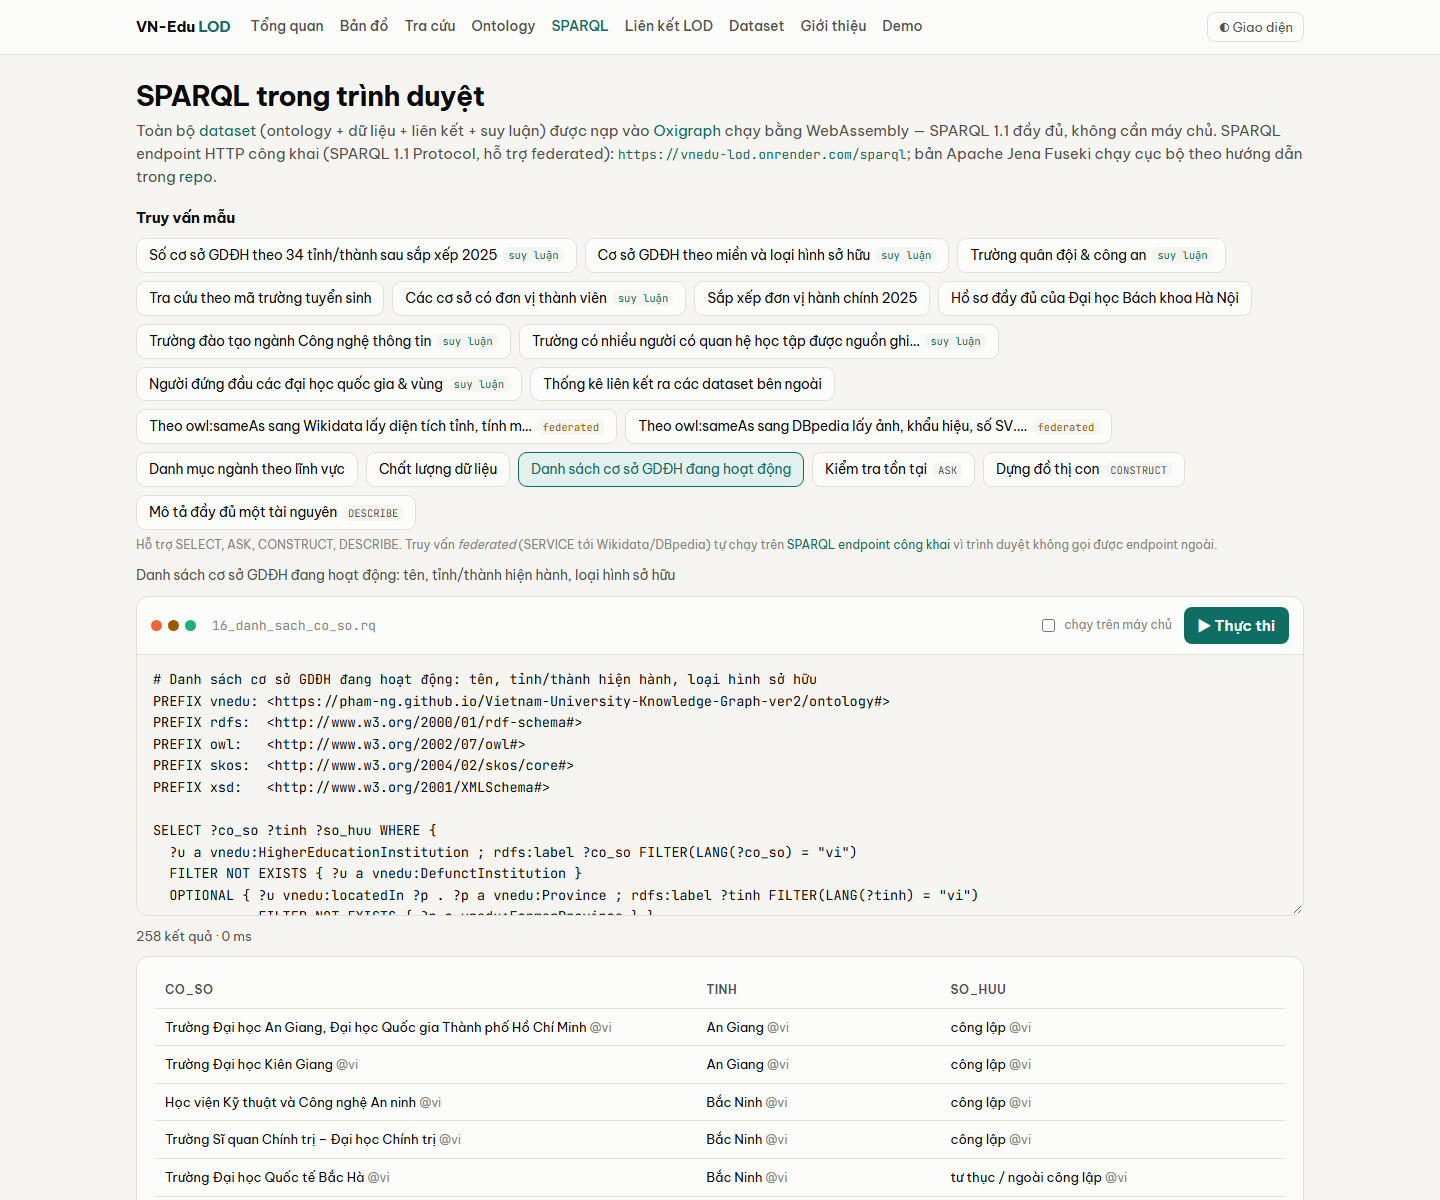
\includegraphics[width=\textwidth]{figures/gen/web-sparql.png}\caption{SPARQL với truy vấn mẫu}\end{subfigure}
\\[6pt]
\begin{subfigure}[t]{0.49\textwidth}\centering
  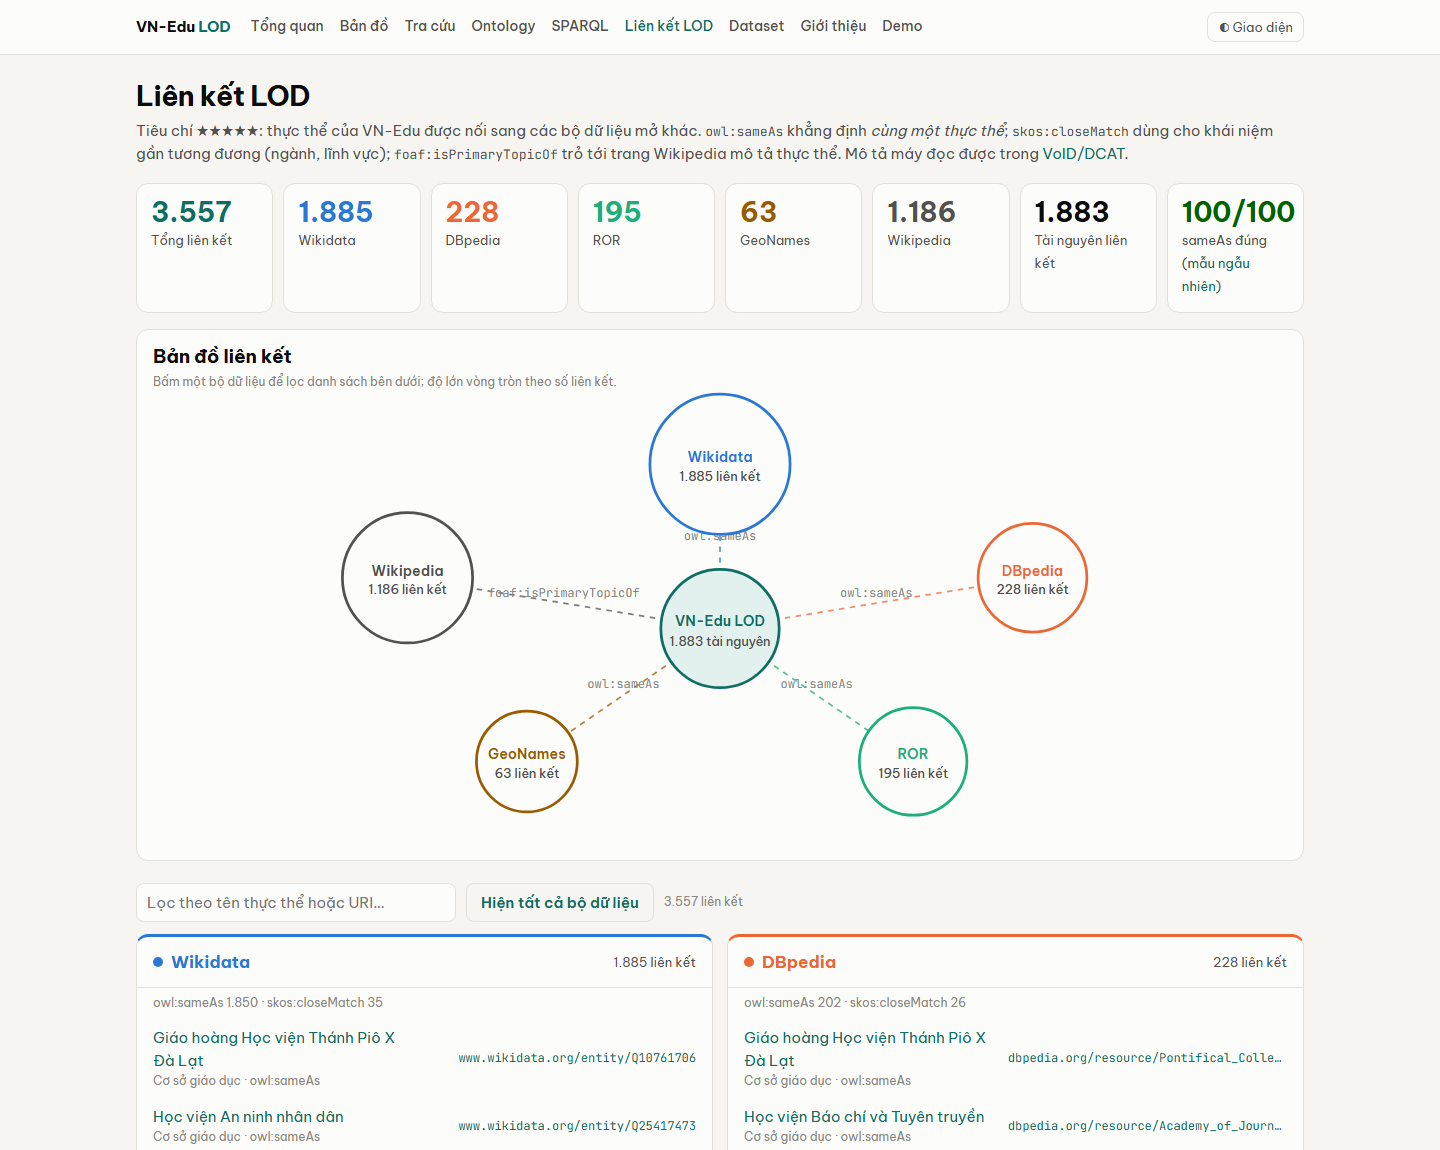
\includegraphics[width=\textwidth]{figures/gen/web-links.png}\caption{Trang Liên kết LOD}\end{subfigure}\hfill
\begin{subfigure}[t]{0.49\textwidth}\centering
  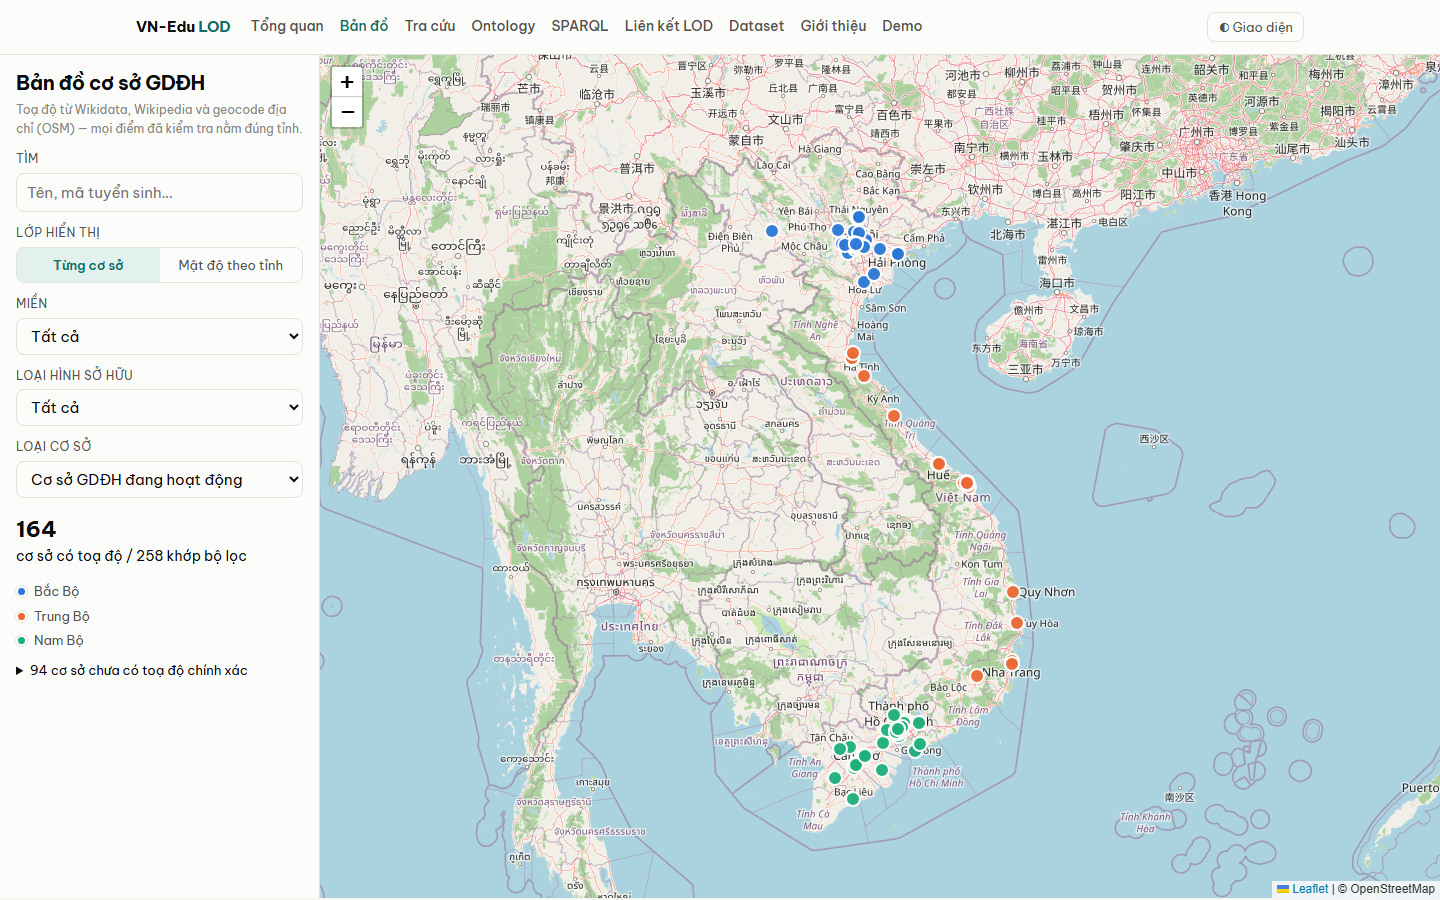
\includegraphics[width=\textwidth]{figures/gen/web-map.png}\caption{Bản đồ cơ sở}\end{subfigure}
\caption{Giao diện web của \proj{}.}\label{fig:web}
\end{figure}

\subsection{Tích hợp liên tục và giám sát}
GitHub Actions chạy ba quy trình: (1) \emph{CI \& Pages}: kiểm định SHACL, suy luận lại và so sánh, kiểm tra số triple
của đồ thị hợp, kiểm thử tải giới hạn và bảo mật của máy chủ, chạy bộ kiểm thử, sau đó xây và triển khai trang tĩnh;
(2) \emph{Fuseki TDB2 acceptance}: tải Fuseki chính thức (có kiểm tra checksum), nạp đồ thị vào TDB2, so khớp kết quả
truy vấn với rdflib, khởi động lại và xác nhận các thao tác ghi bị từ chối; (3) \emph{Public endpoint monitor}: định kỳ
kiểm tra trang tĩnh và endpoint trên Render.

% ================================================================= 9. ĐÁNH GIÁ
\section{Đánh giá}\label{sec:eval}

\subsection{Thống kê đồ thị}
\begin{table}[htbp]
\centering\small
\caption{Thống kê bản phát hành (sinh bởi \texttt{audit/release\_metrics.py}).}\label{tab:stats}
\begin{tabular}{lr@{\hspace{1.5cm}}lr}
\toprule
Thực thể & Số lượng & Đồ thị & Triple \\
\midrule
Cơ sở giáo dục & \metricInstitutions & Dữ liệu khẳng định & \metricAssertedTriples \\
\quad trong đó cơ sở GDĐH & \metricHEIs & \quad trong đó siêu dữ liệu quan sát & 35{,}538 \\
\quad đang hoạt động / đã giải thể & 258 / 10 & Liên kết & \metricLinkTriples \\
Cá nhân & \metricPeople & Suy luận & \metricInferredTriples \\
\quad người học (EducationParticipant) & \metricEducationParticipants & Toạ độ OSM & \metricOsmCoordinateTriples \\
\quad lãnh đạo / người đứng đầu & \metricLeaders{} / 198 & Ontology & \metricOntologyTriples \\
Cơ quan chủ quản & 50 & VoID/DCAT & \metricMetadataTriples \\
Tỉnh hiện hành / tỉnh cũ / miền & 34 / 29 / 3 & \textbf{Tổng (đồ thị hợp)} & \textbf{\metricUnionTriples} \\
Ngành / lĩnh vực / chương trình & \metricMajors{} / 16 / \metricPrograms & URI cục bộ & \metricLocalResources \\
\bottomrule
\end{tabular}
\end{table}

Phân bố cơ sở GDĐH đang hoạt động theo miền và loại hình sở hữu (\cref{fig:region}) cho thấy Bắc Bộ chiếm khoảng 50\%.
Khu vực tư thục tập trung ở Nam Bộ (16 so với 10 ở Bắc Bộ). Phân bố năm thành lập (\cref{fig:decades}) có hai đỉnh: thập
niên 1950--1960 (xây dựng hệ thống ở miền Bắc) và thập niên 2000 (mở rộng xã hội hoá giáo dục).

\begin{figure}[htbp]
\centering
\begin{subfigure}[t]{0.48\textwidth}\centering
\begin{tikzpicture}
\begin{axis}[ybar stacked, width=\textwidth, height=6cm, bar width=18pt, ymin=0,
  symbolic x coords={Bắc,Trung,Nam}, xtick=data, ylabel={Số cơ sở}, enlarge x limits=0.25,
  legend style={font=\scriptsize, at={(0.98,0.98)}, anchor=north east, draw=none, fill=white, fill opacity=0.85},
  axis lines*=left, ymajorgrids, grid style={black!10}, tick label style={font=\small}]
\addplot[fill=s1!75, draw=s1] coordinates {(Bắc,\stBacPub) (Trung,\stTrungPub) (Nam,\stNamPub)};
\addplot[fill=s2!75, draw=s2] coordinates {(Bắc,\stBacPri) (Trung,\stTrungPri) (Nam,\stNamPri)};
\addplot[fill=s3!75, draw=s3] coordinates {(Bắc,\stBacRel) (Trung,\stTrungRel) (Nam,\stNamRel)};
\addplot[fill=s4!50, draw=s4] coordinates {(Bắc,\stBacUnk) (Trung,\stTrungUnk) (Nam,\stNamUnk)};
\legend{Công lập, Tư thục, Tôn giáo/khác, Chưa rõ}
\end{axis}
\end{tikzpicture}
\caption{Theo miền và loại hình sở hữu (\stActiveHEI{} cơ sở đang hoạt động).}\label{fig:region}
\end{subfigure}\hfill
\begin{subfigure}[t]{0.5\textwidth}\centering
\begin{tikzpicture}
\begin{axis}[ybar, width=\textwidth, height=6cm, bar width=7pt, ymin=0,
  xlabel={Thập niên thành lập}, ylabel={Số cơ sở}, xtick={1890,1910,...,2020},
  x tick label style={rotate=45, anchor=east, font=\scriptsize, /pgf/number format/1000 sep={}},
  axis lines*=left, ymajorgrids, grid style={black!10}, enlarge x limits=0.05]
\addplot[fill=acc!70, draw=acc] coordinates {\stDecades};
\end{axis}
\end{tikzpicture}
\caption{Theo thập niên thành lập.}\label{fig:decades}
\end{subfigure}
\caption{Hai phân bố trả lời câu hỏi \CQ{2} (sinh trực tiếp từ đồ thị bằng SPARQL).}\label{fig:dist}
\end{figure}

\subsection{Độ phủ dữ liệu}
\Cref{fig:coverage} cho biết tỉ lệ trong \metricInstitutions{} cơ sở có giá trị cho từng thuộc tính. Các thuộc tính cốt
lõi (tỉnh, năm thành lập, website, loại hình) đạt 86--96\%. Toạ độ đạt 59\% (175/297), và quy mô sinh viên chỉ 9\%
(28/297) vì nguồn mở hiếm khi công bố số liệu này.

\begin{figure}[htbp]
\centering
\begin{tikzpicture}
\begin{axis}[xbar, width=0.78\textwidth, height=6.4cm, bar width=9pt, xmin=0, xmax=100,
  symbolic y coords={Số sinh viên,Toạ độ,Mã tuyển sinh,Loại hình sở hữu,Website,Năm thành lập,Tỉnh/thành},
  ytick=data, xlabel={\% trong 297 cơ sở}, nodes near coords={\pgfmathprintnumber[precision=0]{\pgfplotspointmeta}\%},
  every node near coord/.append style={font=\scriptsize}, axis lines*=left, xmajorgrids, grid style={black!10},
  enlarge y limits=0.1]
\addplot[fill=s3!70, draw=s3] coordinates {(9.4,Số sinh viên) (58.9,Toạ độ) (74.1,Mã tuyển sinh)
  (85.9,Loại hình sở hữu) (86.9,Website) (92.9,Năm thành lập) (96.0,Tỉnh/thành)};
\end{axis}
\end{tikzpicture}
\caption{Độ phủ thuộc tính trên 297 cơ sở giáo dục.}\label{fig:coverage}
\end{figure}

\subsection{Độ chính xác liên kết}
Để đánh giá liên kết \texttt{owl:sameAs}, \texttt{audit/link\_precision.py} rút ngẫu nhiên phân tầng 100 liên kết từ
toàn bộ liên kết đã phát hành (seed 20261009; Wikidata 60, DBpedia 20, ROR 10, GeoNames 10). Mỗi liên kết được đối chiếu
với siêu dữ liệu của \emph{chính đích}, không dùng đầu ra của bộ liên kết: loại thực thể phải tương thích (Wikidata
\texttt{P31}, \texttt{rdf:type} của DBpedia, loại của ROR, \texttt{featureCode} của GeoNames), tên phải khớp, và với
người thì năm sinh phải trùng. 93 liên kết qua kiểm tra tự động. 7 liên kết còn lại được đánh giá thủ công, có ghi bằng
chứng trong \texttt{data/reference/link\_precision\_review.csv}. Kết quả: 100/100 đúng (\cref{tab:precision}).

\begin{table}[htbp]
\centering\small
\caption{Độ chính xác liên kết \texttt{owl:sameAs} theo tầng (mẫu ngẫu nhiên phân tầng).}\label{tab:precision}
\begin{tabular}{lrrrl}
\toprule
Tầng & Số liên kết & Mẫu & Đúng & Wilson 95\% \\
\midrule
Wikidata & 1{,}850 & 60 & 60 & 94,0--100\% \\
DBpedia  & 202 & 20 & 20 & 83,9--100\% \\
ROR      & 195 & 10 & 10 & 72,2--100\% \\
GeoNames & 63  & 10 & 10 & 72,2--100\% \\
\midrule
Tổng     & 2{,}310 & 100 & 100 & 96,3--100\% \\
\bottomrule
\end{tabular}
\end{table} Với \(n=100\) và
\(\hat p=1\), khoảng tin cậy Wilson~\cite{wilson1927} 95\% là
\[
\left[\frac{n}{n+z^2}\left(\hat p + \frac{z^2}{2n} - z\sqrt{\frac{\hat p(1-\hat p)}{n}+\frac{z^2}{4n^2}}\right),\,1\right]
= [0{,}963;\ 1],\qquad z=1{,}96 .
\]
Chúng tôi dùng khoảng Wilson thay vì khoảng Wald vì khoảng Wald suy biến thành \([1;1]\) khi \(\hat p = 1\). Độ chính
xác cao này đến từ chính sách bảo thủ: chỉ chấp nhận QID do nguồn ghi nhận hoặc khớp chính xác, và chỉ chấp nhận
DBpedia khi ánh xạ là một--một. Đổi lại, độ phủ giảm: 228 liên kết DBpedia so với 1{,}885 liên kết Wikidata.

\subsection{Hiệu năng}
\begin{table}[htbp]
\centering\small
\caption{Độ trễ đo được (trung vị 5 lần chạy). Render: gói miễn phí, CPU dùng chung, máy đã khởi động.}\label{tab:perf}
\begin{tabular}{llrr}
\toprule
Kênh & Thao tác & Cục bộ & Render \\
\midrule
Trình duyệt (Oxigraph/WASM) & nạp \metricUnionTriples{} triple (5~MB) & 0,24 s & -- \\
                            & truy vấn mẫu & 83--111 ms & -- \\
Máy chủ (rdflib)            & Q01 tổng hợp theo 34 tỉnh (suy luận) & 0,34 s & 1,59 s \\
                            & Q02 miền \(\times\) loại hình & 0,23 s & 1,31 s \\
                            & Q03 trường quân đội, công an & 0,15 s & 0,90 s \\
                            & Q09 xếp hạng cựu sinh viên & 0,53 s & 3,61 s \\
                            & Q16 danh sách cơ sở & 0,66 s & 4,48 s \\
                            & tra cứu URI (Turtle) & 3 ms & 85 ms \\
\bottomrule
\end{tabular}
\end{table}

Trên Render, độ trễ cao hơn 4--7 lần so với chạy cục bộ do CPU dùng chung. Các truy vấn vẫn chạy dưới 5 giây, đủ dùng
cho mục đích tra cứu. Khi máy ngủ (cold start), yêu cầu đầu tiên mất 30--60 giây; vì vậy trang tĩnh với Oxigraph là
kênh chính cho người dùng.

\subsection{Tái lập và kiểm thử}
\begin{itemize}
  \item \textbf{Tái lập}: hai lần chạy \texttt{VNEDU\_OFFLINE=1 python run\_all.py} liên tiếp trên hai thư mục sạch sinh
  ra các tệp Gold có SHA-256 giống nhau. Có được điều này là nhờ ghi Turtle theo thứ tự tất định, thời gian phát hành cố
  định, và không phụ thuộc thứ tự duyệt \texttt{set}.
  \item \textbf{Kiểm thử}: 202 ca kiểm thử pytest bao phủ trích xuất, hợp đồng dữ liệu Silver, suy luận (mỗi lớp định
  nghĩa có ca kiểm thử dương tính và âm tính), SHACL, máy chủ (thương lượng nội dung, 406, CORS, chặn
  \texttt{UPDATE}, chặn \texttt{SERVICE} ngoài danh sách cho phép, chống XSS trong liên kết), và các lỗi hồi quy đã sửa.
\end{itemize}

\subsection{Trả lời câu hỏi nghiên cứu}
\begin{description}[leftmargin=1.2cm,style=nextline]
  \item[\RQ{1}] Có. Ontology 2.4 biểu đạt được mọi câu hỏi năng lực ở \cref{tab:cq}; nằm trong cả OWL~2~RL và OWL~2~DL;
  vật chất hoá toàn bộ dữ liệu trong vài giây. Các khái niệm đặc thù Việt Nam (chủ quản, sáp nhập tỉnh) được xử lý bằng
  lớp định nghĩa và chuỗi thuộc tính thay vì mã thủ tục.
  \item[\RQ{2}] Có. Bộ đệm HTTP và Medallion bảo đảm tái lập byte. \texttt{field\_sources} và \texttt{SourceObservation}
  bảo đảm mọi giá trị đều có nguồn và các mâu thuẫn được giữ lại.
  \item[\RQ{3}] Có. Bộ dữ liệu đáp ứng đủ 5 tiêu chí (\cref{tab:5star}), có độ chính xác liên kết \(\geq 96{,}3\%\) (cận
  dưới Wilson) và dịch vụ truy cập miễn phí với độ trễ dưới 5 giây.
\end{description}

% ================================================================= 10. THẢO LUẬN
\section{Thảo luận và hạn chế}\label{sec:discussion}

\paragraph{Đe doạ tính hợp lệ.}
\begin{itemize}
  \item \textbf{Mẫu kiểm tra liên kết nhỏ, một người đánh giá}: 100 liên kết chỉ cho cận dưới 96,3\%. Các tầng nhỏ
  (ROR, GeoNames) có cận dưới chỉ 72\%. Chưa có người đánh giá thứ hai để đo độ đồng thuận (Cohen \(\kappa\)). Với 2{,}310 liên kết \texttt{sameAs},
  vẫn có thể còn tới khoảng 85 liên kết sai mà mẫu không phát hiện được. Đánh giá chỉ đo \emph{độ chính xác}, chưa đo
  \emph{độ phủ} (recall) vì không có tập chuẩn đầy đủ.
  \item \textbf{Phụ thuộc vào nguồn cộng đồng}: thông tin lãnh đạo và người học phần lớn đến từ Wikidata và Wikipedia.
  Mô hình \texttt{SourceObservation} giúp không khẳng định sai thời điểm, nhưng không sửa được chính nguồn khi nguồn sai.
  \item \textbf{Thời điểm chụp}: dữ liệu phản ánh thời điểm thu thập (tháng 10/2026). Ví dụ, số điện thoại của ĐHBK Hà
  Nội trong dữ liệu (024 3869 6099, lấy từ MOET) khác số trên trang chính thức hiện tại (024 3869 4242).
\end{itemize}

\paragraph{Hạn chế về phạm vi.}
\begin{itemize}
  \item \textbf{Đơn vị cấp dưới}: ontology có \vn{UniversitySchool} và \vn{memberOf}, nhưng dữ liệu chưa có các trường
  và khoa trực thuộc \emph{bên trong} một đại học. Ví dụ, ĐHBK Hà Nội có 6 trường và 7 khoa (Trường Công nghệ Thông tin
  và Truyền thông, Trường Cơ khí\dots) nhưng các đơn vị này chưa có trong đồ thị, vì Wikidata và MOET không mô tả cấp
  này. Mở rộng sẽ cần thu thập từ trang của từng trường. Việc mở rộng không ảnh hưởng tới mức 5 sao, với điều kiện mỗi
  đơn vị mới vẫn có URI tra cứu được và có nguồn.
  \item \textbf{Chương trình đào tạo}: hiện chỉ có 78 chương trình mẫu, chưa phải toàn bộ danh mục.
  \item \textbf{Không dùng 303}: URI sự vật trả trực tiếp biểu diễn (kèm \texttt{Vary: Accept}) thay vì chuyển hướng
  303 như khuyến nghị Cool URIs, do ràng buộc của GitHub Pages.
  \item \textbf{Hạ tầng}: gói miễn phí của Render ngủ khi không có truy cập; rdflib trong bộ nhớ không phù hợp với đồ thị
  lớn hơn vài triệu triple.
\end{itemize}

\paragraph{Bài học.} (1) Ranh giới giữa \emph{điều nguồn nói} và \emph{điều đang đúng} phải được mô hình hoá rõ ràng
ngay từ đầu, vì đây là điểm yếu phổ biến nhất của các bộ LOD trích từ Wikipedia. (2) Chọn OWL~2~RL giúp đưa suy luận vào
pipeline một cách rẻ và có thể kiểm thử. (3) Liên kết \texttt{sameAs} ra ngoài cần được cô lập khỏi bước suy luận.

% ================================================================= 11. KẾT LUẬN
\section{Kết luận và hướng phát triển}\label{sec:conclusion}
Đồ án đã xây dựng \proj{}, một ứng dụng dữ liệu liên kết mở 5 sao về giáo dục đại học Việt Nam. Ứng dụng gồm: ontology
OWL~2 có kiểm chứng bằng bộ suy luận; pipeline Medallion tái lập được; \metricUnionTriples{} triple có nguồn gốc rõ ràng;
\metricLinkTriples{} liên kết ra ngoài với độ chính xác được đo; và hai kênh công bố tuân thủ chuẩn W3C. Điểm khác biệt
so với các đồ án tham khảo là cách tiếp cận \emph{có bằng chứng}: mỗi khẳng định có nguồn, mỗi mâu thuẫn được giữ lại,
mỗi chỉ số trong báo cáo được sinh tự động từ dữ liệu.

Các hướng phát triển gồm:
\begin{enumerate}
  \item Bổ sung các đơn vị cấp dưới (trường, khoa trực thuộc đại học) và lãnh đạo của các đơn vị này.
  \item Đồng bộ định kỳ với Wikidata. Có thể đóng góp ngược các liên kết ROR/GeoNames và mã tuyển sinh lên Wikidata.
  \item Mở rộng chương trình đào tạo theo danh mục đầy đủ và chỉ tiêu tuyển sinh theo năm, dùng
  \vn{MeasurementObservation} có \vn{referenceYear}.
  \item Xây dựng hỏi đáp ngôn ngữ tự nhiên trên đồ thị (KGQA hoặc GraphRAG) dùng SPARQL làm lớp truy xuất có kiểm chứng.
\end{enumerate}

% ================================================================= TÀI LIỆU
\clearpage
\phantomsection\addcontentsline{toc}{section}{Tài liệu tham khảo}
\bibliographystyle{plainnat}
\bibliography{references}

% ================================================================= PHỤ LỤC
\clearpage
\appendix
\section{Bảng thuộc tính của ontology}\label{app:properties}
{\small\setlength{\tabcolsep}{3pt}
\begin{longtable}{>{\raggedright\arraybackslash}p{2.5cm}>{\raggedright\arraybackslash}p{2.7cm}>{\raggedright\arraybackslash}p{3.6cm}>{\raggedright\arraybackslash}p{3.0cm}>{\raggedright\arraybackslash}p{2.7cm}}
\caption{Các thuộc tính của ontology \texttt{vnedu:} 2.4 (sinh tự động từ \texttt{ontology/vnedu.ttl}).}\label{tab:props}\\
\toprule
Thuộc tính & Nhãn & Miền \(\rightarrow\) đích & Đặc tính & Căn chỉnh \\
\midrule\endfirsthead
\toprule
Thuộc tính & Nhãn & Miền \(\rightarrow\) đích & Đặc tính & Căn chỉnh \\
\midrule\endhead
\bottomrule\endfoot
\multicolumn{5}{l}{\textbf{Tổ chức và quản trị}} \\
\texttt{governed\allowbreak{}By} & có cơ quan chủ quản & Educational\allowbreak{}Organization \(\rightarrow\) Governing\allowbreak{}Body & nghịch đảo \texttt{governs}; chuỗi \(\mathit{governed\allowbreak{}By}\circ\mathit{subordinate\allowbreak{}To}\) & -- \\
\texttt{directly\allowbreak{}Governed\allowbreak{}By} &  & Educational\allowbreak{}Organization \(\rightarrow\) Governing\allowbreak{}Body & \(\sqsubseteq\) \texttt{governed\allowbreak{}By} & -- \\
\texttt{reported\allowbreak{}Governed\allowbreak{}By} &  & Educational\allowbreak{}Organization \(\rightarrow\) Governing\allowbreak{}Body & \(\sqsubseteq\) \texttt{governed\allowbreak{}By} & -- \\
\texttt{governs} & là cơ quan chủ quản của & Governing\allowbreak{}Body \(\rightarrow\) Educational\allowbreak{}Organization & nghịch đảo \texttt{governed\allowbreak{}By} & -- \\
\texttt{state\allowbreak{}Managed\allowbreak{}By} & chịu quản lý nhà nước của & Educational\allowbreak{}Organization \(\rightarrow\) Governing\allowbreak{}Body & -- & -- \\
\texttt{subordinate\allowbreak{}To} & trực thuộc (cơ quan cấp trên) & Governing\allowbreak{}Body \(\rightarrow\) Governing\allowbreak{}Body & bắc cầu & -- \\
\texttt{owned\allowbreak{}By} & thuộc sở hữu / đầu tư của & Educational\allowbreak{}Organization \(\rightarrow\) Company & -- & -- \\
\texttt{ownership} & loại hình sở hữu & Educational\allowbreak{}Organization \(\rightarrow\) Ownership\allowbreak{}Type & hàm & -- \\
\texttt{member\allowbreak{}Of} & là thành viên của & Educational\allowbreak{}Organization \(\rightarrow\) Higher\allowbreak{}Education\allowbreak{}Institution & nghịch đảo \texttt{has\allowbreak{}Member} & -- \\
\texttt{has\allowbreak{}Member} & có đơn vị thành viên & Higher\allowbreak{}Education\allowbreak{}Institution \(\rightarrow\) Educational\allowbreak{}Organization & nghịch đảo \texttt{member\allowbreak{}Of} & -- \\
\texttt{branch\allowbreak{}Of} & là phân hiệu của & Branch \(\rightarrow\) Higher\allowbreak{}Education\allowbreak{}Institution & hàm; nghịch đảo \texttt{has\allowbreak{}Branch} & \texttt{schema:\allowbreak{}parent\allowbreak{}Organization} \\
\texttt{has\allowbreak{}Branch} & có phân hiệu & Higher\allowbreak{}Education\allowbreak{}Institution \(\rightarrow\) Branch & nghịch đảo \texttt{branch\allowbreak{}Of} & \texttt{schema:\allowbreak{}sub\allowbreak{}Organization} \\
\texttt{predecessor} & tiền thân & Educational\allowbreak{}Organization \(\rightarrow\) Organization & nghịch đảo \texttt{successor} & \texttt{dbo:\allowbreak{}predecessor} \\
\texttt{successor} & đơn vị kế tục & Organization \(\rightarrow\) Organization & nghịch đảo \texttt{predecessor} & \texttt{dbo:\allowbreak{}successor} \\
\texttt{website} & trang web & Organization \(\rightarrow\) -- & -- & \texttt{foaf:\allowbreak{}homepage} \\
\midrule
\multicolumn{5}{l}{\textbf{Lãnh đạo và con người}} \\
\texttt{has\allowbreak{}Leader} & có lãnh đạo được nguồn ghi nhận & Organization \(\rightarrow\) Person & nghịch đảo \texttt{leads} & -- \\
\texttt{leads} & đứng đầu & Person \(\rightarrow\) Organization & nghịch đảo \texttt{has\allowbreak{}Leader} & -- \\
\texttt{has\allowbreak{}Head} & có người đứng đầu & Educational\allowbreak{}Organization \(\rightarrow\) Person & nghịch đảo \texttt{head\allowbreak{}Of}; \(\sqsubseteq\) \texttt{has\allowbreak{}Leader} & -- \\
\texttt{head\allowbreak{}Of} & đứng đầu (theo pháp luật) & Person \(\rightarrow\) Educational\allowbreak{}Organization & nghịch đảo \texttt{has\allowbreak{}Head} & -- \\
\texttt{rector} & hiệu trưởng & Educational\allowbreak{}Organization \(\rightarrow\) Person & \(\sqsubseteq\) \texttt{has\allowbreak{}Head} & \texttt{dbo:\allowbreak{}rector} \\
\texttt{director} & giám đốc & Educational\allowbreak{}Organization \(\rightarrow\) Person & \(\sqsubseteq\) \texttt{has\allowbreak{}Head} & -- \\
\texttt{council\allowbreak{}Chair} & chủ tịch hội đồng trường & Educational\allowbreak{}Organization \(\rightarrow\) Person & \(\sqsubseteq\) \texttt{has\allowbreak{}Leader} & \texttt{dbo:\allowbreak{}chairman} \\
\texttt{educated\allowbreak{}At} & được ghi nhận học tại & Person \(\rightarrow\) Educational\allowbreak{}Organization & nghịch đảo \texttt{has\allowbreak{}Education\allowbreak{}Participant} & -- \\
\texttt{has\allowbreak{}Education\allowbreak{}Participant} &  & Educational\allowbreak{}Organization \(\rightarrow\) Person & nghịch đảo \texttt{educated\allowbreak{}At} & -- \\
\texttt{alumnus\allowbreak{}Of} & cựu sinh viên của & Person \(\rightarrow\) Educational\allowbreak{}Organization & nghịch đảo \texttt{has\allowbreak{}Alumnus} & \texttt{schema:\allowbreak{}alumni\allowbreak{}Of} \\
\texttt{has\allowbreak{}Alumnus} & có cựu sinh viên & Educational\allowbreak{}Organization \(\rightarrow\) Person & nghịch đảo \texttt{alumnus\allowbreak{}Of} & -- \\
\texttt{born\allowbreak{}In} & sinh ra tại (đơn vị hành chính) & Person \(\rightarrow\) Administrative\allowbreak{}Unit & -- & -- \\
\texttt{birth\allowbreak{}Area\allowbreak{}In\allowbreak{}Current\allowbreak{}Crosswalk} &  & Person \(\rightarrow\) Geographic\allowbreak{}Area & chuỗi \(\mathit{born\allowbreak{}In}\circ\mathit{merged\allowbreak{}Into}\); chuỗi \(\mathit{born\allowbreak{}In}\circ\mathit{part\allowbreak{}Of}\); chuỗi \(\mathit{birth\allowbreak{}Area\allowbreak{}In\allowbreak{}Current\allowbreak{}Crosswalk}\circ\mathit{part\allowbreak{}Of}\) & -- \\
\texttt{birth\allowbreak{}Place} & nơi sinh & Person \(\rightarrow\) -- & -- & \texttt{dbo:\allowbreak{}birth\allowbreak{}Place}, \texttt{schema:\allowbreak{}birth\allowbreak{}Place} \\
\texttt{nationality} & quốc tịch & Person \(\rightarrow\) Country & -- & \texttt{dbo:\allowbreak{}nationality}, \texttt{schema:\allowbreak{}nationality} \\
\midrule
\multicolumn{5}{l}{\textbf{Địa lý hành chính}} \\
\texttt{located\allowbreak{}In} & đặt tại & Organization \(\rightarrow\) Geographic\allowbreak{}Area & chuỗi \(\mathit{located\allowbreak{}In}\circ\mathit{part\allowbreak{}Of}\); chuỗi \(\mathit{located\allowbreak{}In}\circ\mathit{merged\allowbreak{}Into}\) & \texttt{schema:\allowbreak{}location} \\
\texttt{part\allowbreak{}Of} & thuộc (khu vực lớn hơn) & Geographic\allowbreak{}Area \(\rightarrow\) Geographic\allowbreak{}Area & bắc cầu; nghịch đảo \texttt{has\allowbreak{}Part} & \texttt{schema:\allowbreak{}contained\allowbreak{}In\allowbreak{}Place} \\
\texttt{has\allowbreak{}Part} & gồm & Geographic\allowbreak{}Area \(\rightarrow\) Geographic\allowbreak{}Area & nghịch đảo \texttt{part\allowbreak{}Of} & \texttt{schema:\allowbreak{}contains\allowbreak{}Place} \\
\texttt{merged\allowbreak{}Into} & sáp nhập vào & Former\allowbreak{}Province \(\rightarrow\) Province & hàm; nghịch đảo \texttt{merged\allowbreak{}From} & -- \\
\texttt{merged\allowbreak{}From} & hình thành từ & Province \(\rightarrow\) Former\allowbreak{}Province & nghịch đảo \texttt{merged\allowbreak{}Into} & -- \\
\midrule
\multicolumn{5}{l}{\textbf{Đào tạo}} \\
\texttt{offers\allowbreak{}Program} & đào tạo chương trình & Educational\allowbreak{}Organization \(\rightarrow\) Academic\allowbreak{}Program & nghịch đảo \texttt{offered\allowbreak{}By} & -- \\
\texttt{offered\allowbreak{}By} & do ... đào tạo & Academic\allowbreak{}Program \(\rightarrow\) Educational\allowbreak{}Organization & nghịch đảo \texttt{offers\allowbreak{}Program} & \texttt{schema:\allowbreak{}provider} \\
\texttt{of\allowbreak{}Major} & thuộc ngành & Academic\allowbreak{}Program \(\rightarrow\) Major & -- & -- \\
\texttt{trains\allowbreak{}Major} & đào tạo ngành & Educational\allowbreak{}Organization \(\rightarrow\) Major & chuỗi \(\mathit{offers\allowbreak{}Program}\circ\mathit{of\allowbreak{}Major}\) & -- \\
\texttt{in\allowbreak{}Field} & thuộc lĩnh vực & Major \(\rightarrow\) Field\allowbreak{}Of\allowbreak{}Study & -- & \texttt{skos:\allowbreak{}broader} \\
\midrule
\multicolumn{5}{l}{\textbf{Thuộc tính dữ liệu}} \\
\texttt{founding\allowbreak{}Year} & năm truyền thống (năm thành lập sớm nhất được ghi nhận) & Organization \(\rightarrow\) xsd:\allowbreak{}integer & hàm & -- \\
\texttt{establishment\allowbreak{}Year} & năm thành lập pháp nhân hiện tại & Organization \(\rightarrow\) xsd:\allowbreak{}integer & hàm & -- \\
\texttt{reported\allowbreak{}Founding\allowbreak{}Date} & ngày thành lập khác được nguồn ghi nhận & Organization \(\rightarrow\) xsd:\allowbreak{}date\allowbreak{}Time & -- & -- \\
\texttt{dissolution\allowbreak{}Year} & năm giải thể / sáp nhập & Organization \(\rightarrow\) xsd:\allowbreak{}integer & hàm & -- \\
\texttt{admission\allowbreak{}Code} & mã trường (tuyển sinh) & Educational\allowbreak{}Organization \(\rightarrow\) xsd:\allowbreak{}string & -- & \texttt{skos:\allowbreak{}notation} \\
\texttt{short\allowbreak{}Name} & tên viết tắt & Organization \(\rightarrow\) xsd:\allowbreak{}string & -- & \texttt{dbo:\allowbreak{}abbreviation} \\
\texttt{former\allowbreak{}Name} & tên cũ & Organization \(\rightarrow\) rdfs:\allowbreak{}Literal & -- & \texttt{dbo:\allowbreak{}former\allowbreak{}Name} \\
\texttt{motto} & khẩu hiệu & Educational\allowbreak{}Organization \(\rightarrow\) rdfs:\allowbreak{}Literal & -- & -- \\
\texttt{address} & địa chỉ & Organization \(\rightarrow\) xsd:\allowbreak{}string & -- & -- \\
\texttt{campus} & khuôn viên & Educational\allowbreak{}Organization \(\rightarrow\) xsd:\allowbreak{}string & -- & -- \\
\texttt{funding} & tài trợ, ngân sách, vốn đầu tư & Educational\allowbreak{}Organization \(\rightarrow\) xsd:\allowbreak{}string & -- & -- \\
\texttt{history} & lịch sử hình thành & Educational\allowbreak{}Organization \(\rightarrow\) rdfs:\allowbreak{}Literal & -- & -- \\
\texttt{foreign\allowbreak{}Invested} & có vốn đầu tư nước ngoài & Educational\allowbreak{}Organization \(\rightarrow\) xsd:\allowbreak{}boolean & hàm & -- \\
\texttt{number\allowbreak{}Of\allowbreak{}Students} & số sinh viên & Educational\allowbreak{}Organization \(\rightarrow\) xsd:\allowbreak{}non\allowbreak{}Negative\allowbreak{}Integer & -- & \texttt{dbo:\allowbreak{}number\allowbreak{}Of\allowbreak{}Students} \\
\texttt{number\allowbreak{}Of\allowbreak{}Undergraduates} & số sinh viên đại học & Educational\allowbreak{}Organization \(\rightarrow\) xsd:\allowbreak{}non\allowbreak{}Negative\allowbreak{}Integer & -- & \texttt{dbo:\allowbreak{}number\allowbreak{}Of\allowbreak{}Undergraduate\allowbreak{}Students} \\
\texttt{number\allowbreak{}Of\allowbreak{}Postgraduates} & số học viên sau đại học & Educational\allowbreak{}Organization \(\rightarrow\) xsd:\allowbreak{}non\allowbreak{}Negative\allowbreak{}Integer & -- & \texttt{dbo:\allowbreak{}number\allowbreak{}Of\allowbreak{}Postgraduate\allowbreak{}Students} \\
\texttt{academic\allowbreak{}Staff} & số giảng viên & Educational\allowbreak{}Organization \(\rightarrow\) xsd:\allowbreak{}non\allowbreak{}Negative\allowbreak{}Integer & -- & \texttt{dbo:\allowbreak{}faculty\allowbreak{}Size} \\
\texttt{population} & dân số & Administrative\allowbreak{}Unit \(\rightarrow\) xsd:\allowbreak{}non\allowbreak{}Negative\allowbreak{}Integer & -- & \texttt{dbo:\allowbreak{}population\allowbreak{}Total} \\
\texttt{area} & diện tích (km²) & Administrative\allowbreak{}Unit \(\rightarrow\) xsd:\allowbreak{}decimal & -- & -- \\
\texttt{birth\allowbreak{}Date} & ngày sinh & Person \(\rightarrow\) xsd:\allowbreak{}date\allowbreak{}Time & hàm & \texttt{schema:\allowbreak{}birth\allowbreak{}Date} \\
\texttt{honorific} & học hàm, học vị, quân hàm & Person \(\rightarrow\) xsd:\allowbreak{}string & -- & \texttt{schema:\allowbreak{}honorific\allowbreak{}Prefix} \\
\texttt{code} & mã ngành / mã lĩnh vực & -- \(\rightarrow\) xsd:\allowbreak{}string & -- & \texttt{skos:\allowbreak{}notation} \\
\texttt{degree\allowbreak{}Level} & trình độ đào tạo & Academic\allowbreak{}Program \(\rightarrow\) rdfs:\allowbreak{}Literal & -- & -- \\
\midrule
\multicolumn{5}{l}{\textbf{Nguồn gốc và thời gian (SourceObservation)}} \\
\texttt{snapshot\allowbreak{}Digest} &  & Source\allowbreak{}Observation \(\rightarrow\) xsd:\allowbreak{}string & -- & -- \\
\texttt{temporal\allowbreak{}Status} &  & Source\allowbreak{}Observation \(\rightarrow\) xsd:\allowbreak{}string & -- & -- \\
\texttt{valid\allowbreak{}From} &  & Source\allowbreak{}Observation \(\rightarrow\) xsd:\allowbreak{}date\allowbreak{}Time & -- & -- \\
\texttt{valid\allowbreak{}Through} &  & Source\allowbreak{}Observation \(\rightarrow\) xsd:\allowbreak{}date\allowbreak{}Time & -- & -- \\
\texttt{reference\allowbreak{}Year} &  & Source\allowbreak{}Observation \(\rightarrow\) xsd:\allowbreak{}integer & -- & -- \\
\texttt{measurement\allowbreak{}Unit} &  & Measurement\allowbreak{}Observation \(\rightarrow\) xsd:\allowbreak{}string & -- & -- \\
\end{longtable}}


\section{Truy vấn SPARQL tiêu biểu}\label{app:queries}
Toàn bộ 19 truy vấn nằm trong thư mục \texttt{queries/} và chạy được bằng \texttt{python query.py <số>}. Mọi truy vấn
dùng tiền tố \texttt{vnedu:} như ở \cref{sec:ontology}.

\codetitle{Q01 -- Số cơ sở GDĐH theo 34 tỉnh mới (dùng chuỗi \texttt{locatedIn} \(\circ\) \texttt{mergedInto})}
\begin{code}
SELECT ?tinh (COUNT(DISTINCT ?u) AS ?so_co_so) (COUNT(DISTINCT ?u_tinh_cu) AS ?trong_do_ghi_o_tinh_cu)
WHERE {
  ?u a vnedu:HigherEducationInstitution ; vnedu:locatedIn ?t .
  ?t a vnedu:Province ; rdfs:label ?tinh FILTER(LANG(?tinh) = "vi")
  OPTIONAL { ?u vnedu:locatedIn ?cu . ?cu vnedu:mergedInto ?t . BIND(?u AS ?u_tinh_cu) }
}
GROUP BY ?tinh ORDER BY DESC(?so_co_so) LIMIT 15
\end{code}

\codetitle{Q03 -- Trường quân đội và công an (lớp định nghĩa)}
\begin{code}
SELECT ?loai ?truong (GROUP_CONCAT(DISTINCT ?cq; separator=", ") AS ?co_quan_truc_tiep)
WHERE {
  VALUES (?c ?loai) { (vnedu:MilitaryInstitution "Quân đội") (vnedu:PoliceInstitution "Công an") }
  ?u a ?c ; rdfs:label ?truong FILTER(LANG(?truong) = "vi")
  OPTIONAL { ?u vnedu:governedBy ?b . ?b rdfs:label ?l FILTER(LANG(?l) = "vi")
             FILTER(?b NOT IN (vnedu:MinistryOfNationalDefence, vnedu:MinistryOfPublicSecurity)) }
  BIND(COALESCE(?l, "—") AS ?cq)
}
GROUP BY ?loai ?truong ORDER BY ?loai ?truong
\end{code}

\codetitle{Q12 -- Truy vấn liên hợp: mật độ trường theo diện tích tỉnh lấy từ Wikidata}
\begin{code}
PREFIX wdt: <http://www.wikidata.org/prop/direct/>
SELECT ?tinh ?so_co_so ?dien_tich_km2 ?co_so_tren_1000km2
WHERE {
  { SELECT ?wd ?tinh (COUNT(DISTINCT ?u) AS ?so_co_so) WHERE {
      ?u a vnedu:HigherEducationInstitution ; vnedu:locatedIn ?t .
      ?t a vnedu:Province ; rdfs:label ?tinh ; owl:sameAs ?wd .
      FILTER(LANG(?tinh) = "vi" && STRSTARTS(STR(?wd), "http://www.wikidata.org/entity/"))
    } GROUP BY ?wd ?tinh ORDER BY DESC(?so_co_so) LIMIT 6 }
  OPTIONAL { SERVICE <https://query.wikidata.org/sparql> { ?wd wdt:P2046 ?dien_tich_km2 } }
  BIND(ROUND(100000 * ?so_co_so / ?dien_tich_km2) / 100 AS ?co_so_tren_1000km2)
}
ORDER BY DESC(?so_co_so)
\end{code}

\section{Hướng dẫn tái lập}\label{app:repro}
\begin{code}
git clone https://github.com/pham-ng/Vietnam-University-Knowledge-Graph-ver2.git
cd Vietnam-University-Knowledge-Graph-ver2
pip install -r requirements.txt
VNEDU_OFFLINE=1 python run_all.py        # xây lại Bronze -> Gold từ bộ đệm, không cần Internet
python -m pytest -q                      # 202 ca kiểm thử
python query.py 1                        # chạy truy vấn Q01 trên đồ thị cục bộ
py app/server.py --prod                  # máy chủ Linked Data (waitress) chạy cục bộ
\end{code}

\end{document}
